\chapter{条件期望}
\label{chap:conditional-expectation}

第~\ref{chap:random-vectors}章已经会算给定一个读数后的平均。两台传感器的概率表中，第一台读$0$时，第二台的平均读数是第一行的加权平均$1/3$；三角形上的均匀分布中，给定$X=x$时$Y$的平均是$x/2$。前者把概率表的一行重新归一，后者把联合密度的一条切片除以它的总积分。

换一个问题，这两种办法都会失效。设$X$在$(-1,1)$上均匀分布，我们只知道它的绝对值$\lvert X\rvert$，想求$X$的正部$X^{+}=\max(X,0)$的平均。知道$\lvert X\rvert=0.6$，就知道$X$是$0.6$或$-0.6$，两者对称，$X^{+}$的平均应当是$0.3$。可是$\{\lvert X\rvert=0.6\}$的概率为零，不能拿它去除；$(X,\lvert X\rvert)$的全部质量落在平面上的两条线段上，也没有联合密度可以切片。直觉给出的答案很清楚，现有的公式却算不出来。

给定的信息也不一定来自某个数值读数。把$[0,1)$等分成四段，只告诉我们样本点落在哪一段，这同样是一份信息；再细分成八段，信息就更多。我们需要一种不依赖概率表或密度、对任意形式的已知信息都能用的条件平均。

本章的办法是不再去除单个条件的概率，而是要求条件平均在每个“已知能否判断其发生”的事件上，保留原变量的累计期望。

第一节从有限分组的组内平均出发，提炼出这一积分刻画，用Radon--Nikodym定理证明它总有解并且几乎必然唯一，再说明给定随机变量时它为何是该变量的函数。第二节在固定的信息下建立线性、保序与提取已知量等运算规则，并讨论独立的信息。第三节研究信息改变时条件平均怎样叠加，得到全期望公式和塔式法则。第四节用凸性比较“先平均再变换”与“先变换再平均”，第五节在平方可积的情形把条件期望解释为最佳预测与正交投影，并把总方差拆成组内与组间两部分。

全章沿用第~\ref{chap:random-vectors}章的两台传感器的概率表作为有限的贯穿例子，用$[0,1)$上$X(\omega)=\omega^{2}$的逐次等分作为连续样本空间上的例子，并用上面的“只知绝对值”作为分组概率为零的例子。比条件平均更完整的对象，即给定信息后的整个条件分布，在第~\ref{chap:conditional-distributions}章建立。

\section{条件期望的定义}
\label{sec:cexp-definition}

第~\ref{chap:random-vectors}章的条件均值都靠除法得到：组内的累计期望除以这一组的概率。只要组的概率为正，这个除法就有意义；一旦条件事件的概率为零，或者根本没有概率表和密度，它就失效。这一节先把有限分组的组内平均重新写成一个随机变量，找出它满足的两条性质；再把这两条性质当作定义，使它在分组概率为零时依然有意义；然后证明这样的随机变量存在而且几乎必然唯一；最后回到给定一个观测的情形，说明条件平均为什么是观测值的函数。

\subsection{有限分组中的条件平均}
\label{sec:cexp-finite-partition}

\paragraph{把组内平均写成随机变量}
回到两台传感器。第一台的档位为$X$，第二台为$Y$，联合概率表见图~\ref{fig:cexp-sensor-rows}(a)。把表中九个格子看作样本空间$\Omega$的九个样本点，每个格子的概率就是表中的数，其中$(0,2)$与$(2,0)$两格的概率为零。$X$与$Y$是这九个点上的函数：格子$(x,y)$上$X=x$，$Y=y$。

\begin{BookInlineFigure}
  \centering
  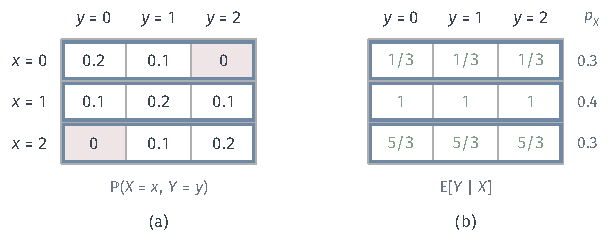
\includegraphics[width=104mm]{figures/07-probability/02-measure-theoretic-probability/tikz/cexp-sensor-rows/figure.pdf}
  \caption{传感器表上的组内平均。(a)九个格子组成样本空间，格中是概率，浅红格的概率为零；蓝框是按$X$的取值分成的三组。(b)随机变量$\mathbb{E}[Y\mid X]$：同一行的每个格子都取这一行$Y$的平均$1/3$、$1$、$5/3$，右侧是各行的概率$p_X$。}
  \label{fig:cexp-sensor-rows}
\end{BookInlineFigure}

知道$X$的值，相当于知道样本点落在哪一行。第~\ref{chap:random-vectors}章算出三行的条件均值$m(0)=1/3$、$m(1)=1$、$m(2)=5/3$。把这三个数填回格子，每一行的所有格子都填该行的均值，就得到图~\ref{fig:cexp-sensor-rows}(b)：一个定义在$\Omega$上的新函数，也就是随机变量$m(X)$。它在样本点$\omega$处的值，是“与$\omega$同组的所有样本点上$Y$的平均”。这个随机变量记作$\mathbb{E}[Y\mid X]$。

这样看，条件平均有两种身份。$m(x)$是一个数，回答“已知$X=x$时$Y$平均是多少”；$\mathbb{E}[Y\mid X]$是一个随机变量，回答“在还不知道结果时，按将来会得到的信息所作的平均是什么”。后者把三个问题的答案一次装进一个对象，本章研究的正是这个对象。

\paragraph{一般的有限分组}
分组不必按某个变量的取值进行。设事件$A_1,\dots,A_k$两两不交，并起来是$\Omega$，称为$\Omega$的一个有限划分。知道“样本点落在哪一组”，就能判断由若干组并成的任何事件是否发生；把这些并集合起来（包括空集），得到
\[
 \mathcal{G}=\Bigl\{\textstyle\bigcup_{i\in S}A_i:\ S\subseteq\{1,\dots,k\}\Bigr\},
\]
它恰好有$2^{k}$个事件。$\mathcal{G}$对补和并封闭，是一个$\sigma$代数，并且是包含$A_1,\dots,A_k$的最小$\sigma$代数。第~\ref{chap:probability-spaces}章用$\sigma$代数表示观测所能区分的信息，$\mathcal{G}$就是“知道所在组”这份信息。按$X$分行时，$\mathcal{G}=\sigma(X)$。

对可积的随机变量$X$，在每个概率为正的组内求平均，再把平均值赋给该组的所有样本点，就得到有限划分下的条件期望：
\begin{equation}
 \mathbb{E}[X\mid\mathcal{G}]=\sum_{i=1}^{k}c_i\mathbf{1}_{A_i},\qquad
 c_i=\frac{\mathbb{E}[X\mathbf{1}_{A_i}]}{\mathbb{P}(A_i)}\quad\text{当}\ \mathbb{P}(A_i)>0 .
 \label{eq:cexp-partition}
\end{equation}
$c_i$正是第~\ref{chap:classical-probability}章“缩小样本范围再重新归一”的平均：把$X$限制在$A_i$上求期望，再除以$A_i$的概率。$\mathbb{P}(A_i)=0$的组没有可以除的数，$c_i$任取一个常数。

\paragraph{概率为零的组}
按读数之差$D=X-Y$分组，就会遇到这种组。$D$取$-2,-1,0,1,2$五个值，对应传感器表的五条对角线，见图~\ref{fig:cexp-difference-groups}(a)。$D=2$与$D=-2$各只含一个概率为零的格子：两台读数从不相差两档。

\begin{BookInlineFigure}
  \centering
  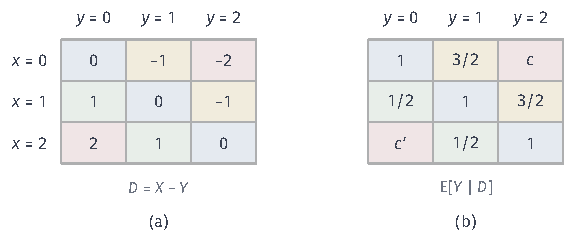
\includegraphics[width=96mm]{figures/07-probability/02-measure-theoretic-probability/tikz/cexp-difference-groups/figure.pdf}
  \caption{按读数之差$D=X-Y$分组。(a)每个格子所属的组，同色格子同组；浅红的两组$D=\pm2$概率为零。(b)$\mathbb{E}[Y\mid D]$在三组正概率组上分别取$1$、$1/2$、$3/2$，在两个零概率组上取任意常数$c$、$c'$。}
  \label{fig:cexp-difference-groups}
\end{BookInlineFigure}

由式~\eqref{eq:cexp-partition}逐组计算。$D=0$的三个格子概率都是$0.2$，$Y$分别取$0,1,2$；$D=1$的两个格子是$(1,0)$与$(2,1)$，概率都是$0.1$；$D=-1$的两个格子是$(0,1)$与$(1,2)$。于是
\[
 \begin{gathered}
 c_{D=0}=\frac{0.2\cdot(0+1+2)}{0.6}=1,\\
 c_{D=1}=\frac{0.1\cdot(0+1)}{0.2}=\frac12,\qquad
 c_{D=-1}=\frac{0.1\cdot(1+2)}{0.2}=\frac32 .
 \end{gathered}
\]
两台读数一致时，第二台的平均档位是$1$；第一台比第二台高一档时，第二台偏低，平均$1/2$；反过来平均$3/2$。$D=\pm2$两组上的值没有可算的依据，图~\ref{fig:cexp-difference-groups}(b)记作$c$与$c'$。

\paragraph{两条性质}
式~\eqref{eq:cexp-partition}得到的随机变量$Z=\mathbb{E}[X\mid\mathcal{G}]$有两条性质，它们后面会变成定义。

第一条，$Z$在每一组内取常数，所以只用到“所在组”这份信息。用$\sigma$代数的语言说：对任何实数集合$B$，$\{Z\in B\}$是若干整组的并，属于$\mathcal{G}$，即$Z$是$\mathcal{G}$可测的。反过来，一个$\mathcal{G}$可测的函数也必定在每组内取常数，因为单点集的原像$\{Z=z\}$只能是整组的并。

第二条，$Z$在每个已知事件上保留$X$的累计期望：
\[
 \mathbb{E}[Z\mathbf{1}_{A}]=\mathbb{E}[X\mathbf{1}_{A}],\qquad A\in\mathcal{G}.
\]
证明只需逐组核对。$A$是若干组$A_i$的并，两边都按组拆成和。对$\mathbb{P}(A_i)>0$的组，由$c_i$的定义，
\[
 \mathbb{E}[Z\mathbf{1}_{A_i}]=c_i\,\mathbb{P}(A_i)=\mathbb{E}[X\mathbf{1}_{A_i}] .
\]
对$\mathbb{P}(A_i)=0$的组，$\mathbf{1}_{A_i}$只在零概率集上非零，两边都是$0$，与$c_i$怎样选无关。把各组相加，就得到上式。

用$D$分组核对一次。取$A=\{D=0\}\cup\{D=1\}$。$Y$在这五个格子上的累计期望为
\[
 \mathbb{E}[Y\mathbf{1}_{A}]=0.2\cdot(0+1+2)+0.1\cdot(0+1)=0.7 ,
\]
而$Z=\mathbb{E}[Y\mid D]$在其中三格取$1$、两格取$1/2$，
\[
 \mathbb{E}[Z\mathbf{1}_{A}]=1\cdot0.6+\tfrac12\cdot0.2=0.7 .
\]
若把$A$换成含有零概率组的事件，例如再并上$\{D=2\}$，两边都不变，$c'$的取值不起作用。

\paragraph{连续样本空间上的有限分组}
样本空间本身不必有限。取$\Omega=[0,1)$，概率是区间长度，令$X(\omega)=\omega^{2}$。把$[0,1)$等分成$2^{n}$段，记这些区间生成的$\sigma$代数为$\mathcal{G}_n$，它表示“只知道$\omega$落在哪一段”。每段的概率为$2^{-n}>0$，式~\eqref{eq:cexp-partition}直接适用。区间$[a,b)$上的平均为
\[
 \frac{1}{b-a}\int_{a}^{b}\omega^{2}\,\mathrm{d}\omega=\frac{a^{2}+ab+b^{2}}{3}.
\]

取$n=2$，四段是$[0,\tfrac14)$、$[\tfrac14,\tfrac12)$、$[\tfrac12,\tfrac34)$、$[\tfrac34,1)$，代入上式，例如第二段为$(\tfrac1{16}+\tfrac18+\tfrac14)/3=\tfrac{7}{48}$，四段依次得到
\[
 \tfrac{1}{48},\qquad \tfrac{7}{48},\qquad \tfrac{19}{48},\qquad \tfrac{37}{48}.
\]
$\mathbb{E}[X\mid\mathcal{G}_2]$是取这四个值的阶梯函数，见图~\ref{fig:cexp-dyadic-average}(a)。在每一段内，阶梯下方的面积与抛物线下方的面积相等，浅蓝的两块“多出”与“缺少”的面积互相抵消，这正是第二条性质在单个组上的样子。分得越细，阶梯越贴近$X$，见图~\ref{fig:cexp-dyadic-average}(b)：信息越多，条件平均保留的$X$的细节越多。

\begin{BookInlineFigure}
  \centering
  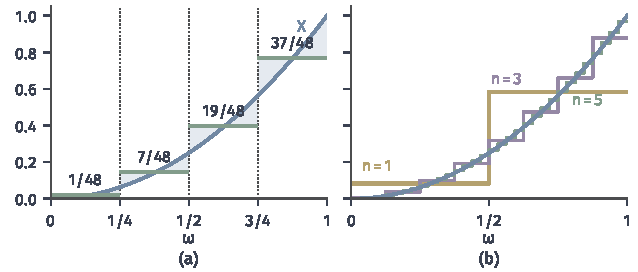
\includegraphics[width=108mm]{figures/07-probability/02-measure-theoretic-probability/matplotlib/cexp-dyadic-average/figure.pdf}
  \caption{$\Omega=[0,1)$上的均匀概率，$X(\omega)=\omega^{2}$（蓝）。(a)$\mathcal{G}_2$由四个等长区间生成，$\mathbb{E}[X\mid\mathcal{G}_2]$（绿）在各段取段内平均；每段内抛物线与阶梯之间的两块浅蓝面积相等。(b)$n=1$（黄）、$n=3$（紫）、$n=5$（绿）时的$\mathbb{E}[X\mid\mathcal{G}_n]$。}
  \label{fig:cexp-dyadic-average}
\end{BookInlineFigure}

\subsection{积分刻画}
\label{sec:cexp-integral}

\paragraph{分组的概率为零时}
回到章首的例子。取$\Omega=(-1,1)$，概率为长度的一半，令$X(\omega)=\omega$，于是$X\sim\operatorname{Unif}(-1,1)$；观测是$Y=\lvert X\rvert$。知道$Y$，就知道样本点在$\{\omega,-\omega\}$这一对之中，所以$\sigma(Y)$把$\Omega$分成不可数多个两点组，每组概率为零。式~\eqref{eq:cexp-partition}一个组也用不上。

直觉的答案是：同组两点概率对称，组内平均就是两点上函数值的算术平均。对正部$X^{+}$，在$\{\omega,-\omega\}$上的两个值是$\lvert\omega\rvert$与$0$，平均为$\lvert\omega\rvert/2$，所以候选答案是
\[
 Z=\frac{Y}{2}=\frac{\lvert X\rvert}{2}.
\]
图~\ref{fig:cexp-folding}(a)画出了它：红色虚线连接$\omega=\pm0.6$处的$X^{+}$，两端的平均$0.3$被赋给这两个点。

\begin{BookInlineFigure}
  \centering
  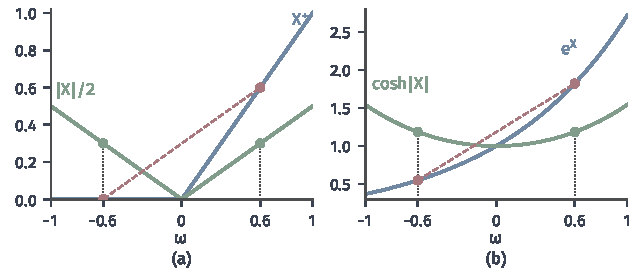
\includegraphics[width=108mm]{figures/07-probability/02-measure-theoretic-probability/matplotlib/cexp-folding/figure.pdf}
  \caption{只知道绝对值时的条件平均，$\Omega=(-1,1)$，$X(\omega)=\omega$均匀分布。(a)$X^{+}$（蓝）与候选的$\mathbb{E}[X^{+}\mid\lvert X\rvert]=\lvert X\rvert/2$（绿）；红点是同组的$\omega=\pm0.6$，两个函数值的平均$0.3$赋给这两点（绿点）。(b)同样地，$\mathrm{e}^{X}$（蓝）的组内平均是$\cosh\lvert X\rvert$（绿）。}
  \label{fig:cexp-folding}
\end{BookInlineFigure}

这个候选不能靠除法检验，但可以用上一小节的第二条性质检验。$\sigma(Y)$中的事件都形如$\{Y\in B\}$，$B\subseteq[0,1)$。$X$的密度在$(-1,1)$上是$\tfrac12$，于是
\[
 \mathbb{E}\bigl[X^{+}\mathbf{1}_{\{Y\in B\}}\bigr]
 =\int_{-1}^{1}\max(x,0)\,\mathbf{1}_{B}(\lvert x\rvert)\,\frac{\mathrm{d}x}{2}
 =\frac12\int_{0}^{1}x\,\mathbf{1}_{B}(x)\,\mathrm{d}x .
\]
另一边，$\lvert x\rvert/2$在$\pm x$处取同一个值，把$(-1,0)$与$(0,1)$两半合并，
\[
 \mathbb{E}\Bigl[\frac{Y}{2}\mathbf{1}_{\{Y\in B\}}\Bigr]
 =\int_{-1}^{1}\frac{\lvert x\rvert}{2}\,\mathbf{1}_{B}(\lvert x\rvert)\,\frac{\mathrm{d}x}{2}
 =\frac12\int_{0}^{1}x\,\mathbf{1}_{B}(x)\,\mathrm{d}x .
\]
两边对每个$B$都相等。候选答案在每个已知事件上保留了$X^{+}$的累计期望，尽管没有一个组可以单独拿来做除法。

\paragraph{定义}
这个例子说明，“在已知事件上保留累计期望”不需要除以组的概率，可以直接拿来作定义；再配上“只用已知信息”这一条，就把有限划分的情形推广到任意的信息。下面固定概率空间$(\Omega,\mathcal{F},\mathbb{P})$和一个$\sigma$代数$\mathcal{G}\subseteq\mathcal{F}$，$\mathcal{G}$表示已知的信息。

\begin{definition}[条件期望]
\label{def:cexp-conditional-expectation}
设$X$是可积的实随机变量，$\mathcal{G}\subseteq\mathcal{F}$是$\sigma$代数。若随机变量$Z$满足：
\begin{enumerate}
 \item $Z$是$\mathcal{G}$可测的；
 \item $Z$可积；
 \item 对每个$A\in\mathcal{G}$，
 \begin{equation}
  \mathbb{E}[Z\mathbf{1}_{A}]=\mathbb{E}[X\mathbf{1}_{A}],
  \label{eq:cexp-defining}
 \end{equation}
\end{enumerate}
则称$Z$为$X$给定$\mathcal{G}$的\term{条件期望}（conditional expectation），记作$\mathbb{E}[X\mid\mathcal{G}]$。满足要求的$Z$可能不止一个，其中每一个都称为\term{条件期望的版本}（version of a conditional expectation）。
\end{definition}

三条要求各有分工。$\mathcal{G}$可测限制了$Z$能用的信息：对每个Borel集$B$，“$Z\in B$是否发生”都必须能由已知事件判断，有限划分时这就是“组内取常数”。可积保证式~\eqref{eq:cexp-defining}左边有意义。式~\eqref{eq:cexp-defining}本身保证每个已知群体的平均不变：当$\mathbb{P}(A)>0$时两边同除以$\mathbb{P}(A)$，它说$Z$与$X$在$A$上的平均相同。

两种极端情形有助于看清定义。若$\mathcal{G}=\{\emptyset,\Omega\}$，什么也不知道，$\mathcal{G}$可测的随机变量只有常数，式~\eqref{eq:cexp-defining}对$A=\Omega$给出常数等于$\mathbb{E}[X]$，所以$\mathbb{E}[X\mid\mathcal{G}]=\mathbb{E}[X]$。若$X$本身是$\mathcal{G}$可测的，什么都已知道，$Z=X$满足全部三条，$\mathbb{E}[X\mid\mathcal{G}]=X$。一般情形介于两者之间：$Z=X$保留了所有累计期望，但通常用了未知的信息；常数$\mathbb{E}[X]$只用已知信息，但只在$A=\Omega$上保留累计期望。条件期望是满足这两方面要求的随机变量。

\paragraph{用定义检验候选}
定义并不给出计算公式，它的作用是检验：先由结构猜出候选，再验证三条要求。用第~\ref{chap:random-vectors}章的三角形模型演示：$(X,Y)$在$\{0\leq y\leq x\leq1\}$上均匀分布，联合密度为$2$。那里算得的条件均值是$m(x)=x/2$，候选为$Z=X/2$。它是$X$的连续函数，所以$\sigma(X)$可测且有界。$\sigma(X)$中的事件形如$\{X\in B\}$，先算$Y$在其上的累计期望，先对$y$积分：
\[
 \mathbb{E}\bigl[Y\mathbf{1}_{\{X\in B\}}\bigr]
 =\int_{B\cap[0,1]}\int_{0}^{x}2y\,\mathrm{d}y\,\mathrm{d}x
 =\int_{B\cap[0,1]}x^{2}\,\mathrm{d}x .
\]
再算候选的累计期望。$X$的边缘密度是$2x$，于是
\[
 \mathbb{E}\Bigl[\frac{X}{2}\mathbf{1}_{\{X\in B\}}\Bigr]
 =\int_{B\cap[0,1]}\frac{x}{2}\cdot2x\,\mathrm{d}x
 =\int_{B\cap[0,1]}x^{2}\,\mathrm{d}x .
\]
两者对每个$B$相等，$X/2$是$\mathbb{E}[Y\mid X]$的一个版本。

错误的候选在定义下会被识别出来。取$B=(-\infty,a]$，$0\leq a\leq1$，正确的累计期望是$a^{3}/3$。若取常数$1/3=\mathbb{E}[Y]$，累计期望变为$\int_0^a\tfrac13\cdot2x\,\mathrm{d}x=a^{2}/3$；若取$X/3$，变为$2a^{3}/9$。前者只在$a=0,1$处与$a^{3}/3$相等，后者在$a=1$处已经不等，见图~\ref{fig:cexp-cumulative-check}。

\begin{BookInlineFigure}
  \centering
  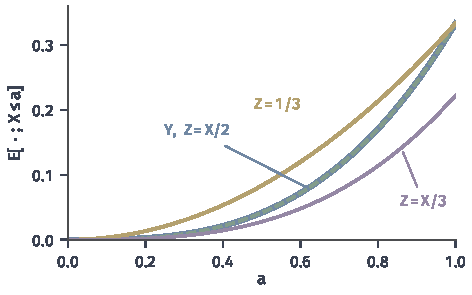
\includegraphics[width=80mm]{figures/07-probability/02-measure-theoretic-probability/matplotlib/cexp-cumulative-check/figure.pdf}
  \caption{用积分刻画检验候选，三角形模型。横轴为$a$，纵轴为事件$\{X\leq a\}$上的累计期望。蓝线是$Y$的$a^{3}/3$，绿色虚线是候选$Z=X/2$，两者重合；黄线是常数候选$1/3$，紫线是候选$X/3$，都与蓝线分离。}
  \label{fig:cexp-cumulative-check}
\end{BookInlineFigure}

\subsection{存在性与唯一性}
\label{sec:cexp-existence}

定义只列出要求，还没有说明满足要求的随机变量是否存在、有几个。有限划分时，式~\eqref{eq:cexp-partition}给出了一个解，零概率组上的任意取值又说明解可能不止一个。一般的$\mathcal{G}$没有组可以逐个处理，需要另找办法。

\paragraph{累计期望是一个测度}
关键是换一个角度看式~\eqref{eq:cexp-defining}的右边。先设$X\geq0$且可积，对$A\in\mathcal{G}$令
\[
 \nu(A)=\mathbb{E}[X\mathbf{1}_{A}] .
\]
$\nu$把每个已知事件对应到$X$在其上的累计期望，可以想成把“$X$的质量”分配到已知事件上。式~\eqref{eq:cexp-defining}要求找一个$\mathcal{G}$可测的$Z$，使$\nu(A)=\mathbb{E}[Z\mathbf{1}_A]$：$Z$是$\nu$相对于$\mathbb{P}$的密度，而且这个密度只能用$\mathcal{G}$中的信息。卷四的Radon--Nikodym定理回答的正是这样的问题：$\sigma$有限测度$\nu$关于$\mu$绝对连续时，存在非负可测函数$h$，使$\nu(A)=\int_A h\,\mathrm{d}\mu$对一切可测集成立，并且$h$在$\mu$几乎处处的意义下唯一，可参考\BookChapterRef{chap:measure-densities}{卷四第8章“测度的密度”}。

图~\ref{fig:cexp-rn-cumulative}用逐次等分的例子展示这个视角。在整个$\mathcal{F}$上，
\[
 \nu([0,t))=\int_0^t\omega^{2}\,\mathrm{d}\omega=\frac{t^{3}}{3},
\]
这条蓝色曲线的斜率就是$X$本身：在$\mathcal{F}$上，$\nu$的密度是$X$。若只允许使用$\mathcal{G}_2$中的事件，$\nu$只在四段及其并上有定义，四段上的质量是
\[
 \begin{gathered}
 \nu(A_1)=\tfrac{1}{192},\qquad \nu(A_2)=\tfrac{7}{192},\\ \nu(A_3)=\tfrac{19}{192},\qquad \nu(A_4)=\tfrac{37}{192},
 \end{gathered}
\]
其中$A_1,\dots,A_4$依次是四个区间。$\mathcal{G}_2$可测的密度在每段上只能取常数，它在$A_i$上必须等于比值$\nu(A_i)/\mathbb{P}(A_i)$，也就是折线在各段的斜率$1/48$、$7/48$、$19/48$、$37/48$，正是第~\ref{sec:cexp-finite-partition}节算出的条件平均。

\begin{BookInlineFigure}
  \centering
  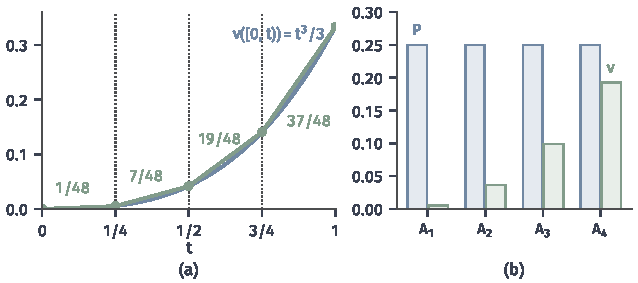
\includegraphics[width=108mm]{figures/07-probability/02-measure-theoretic-probability/matplotlib/cexp-rn-cumulative/figure.pdf}
  \caption{条件期望是限制在$\mathcal{G}$上的密度，$\Omega=[0,1)$，$X(\omega)=\omega^{2}$，$\mathcal{G}=\mathcal{G}_2$。(a)蓝线是$\nu([0,t))=t^{3}/3$，斜率为$X$；绿色折线只经过四个分点，各段斜率是$\mathbb{E}[X\mid\mathcal{G}_2]$的取值。(b)四个区间上$\mathbb{P}(A_i)=1/4$（蓝）与$\nu(A_i)$（绿）的比较，两者之比就是各段斜率。}
  \label{fig:cexp-rn-cumulative}
\end{BookInlineFigure}

\paragraph{存在与唯一}
有了这个视角，存在性归结为在可测空间$(\Omega,\mathcal{G})$上使用Radon--Nikodym定理。唯一性则只用到式~\eqref{eq:cexp-defining}对足够多的事件成立。

\begin{theorem}[条件期望的存在与唯一]
\label{thm:cexp-existence}
设$X$可积，$\mathcal{G}\subseteq\mathcal{F}$是$\sigma$代数。则$X$给定$\mathcal{G}$的条件期望存在。若$Z$与$Z'$都是它的版本，则$Z=Z'$几乎必然成立；反过来，若$Z$是一个版本，$Z'$是$\mathcal{G}$可测的随机变量且$Z'=Z$几乎必然成立，则$Z'$也是一个版本。
\end{theorem}

\begin{proof}
\emph{第一步，非负的$X$。}设$X\geq0$且可积，对$A\in\mathcal{G}$令$\nu(A)=\mathbb{E}[X\mathbf{1}_{A}]$。$\nu(\emptyset)=0$；若$A_1,A_2,\dots\in\mathcal{G}$两两不交，则
\[
 X\mathbf{1}_{\bigcup_nA_n}=\sum_nX\mathbf{1}_{A_n},
\]
右边各项非负，由单调收敛定理，
\[
 \nu\Bigl(\bigcup_nA_n\Bigr)=\sum_n\nu(A_n).
\]
所以$\nu$是$(\Omega,\mathcal{G})$上的测度，总质量$\nu(\Omega)=\mathbb{E}[X]<\infty$。

记$\mathbb{P}_{\mathcal{G}}$为$\mathbb{P}$限制在$\mathcal{G}$上得到的概率测度。若$A\in\mathcal{G}$且$\mathbb{P}(A)=0$，则$X\mathbf{1}_{A}$只在零概率集上非零，$\nu(A)=0$，即$\nu\ll\mathbb{P}_{\mathcal{G}}$。两个测度都有限，由Radon--Nikodym定理，存在$\mathcal{G}$可测的$Z:\Omega\to[0,\infty)$，使
\[
 \nu(A)=\int_{A}Z\,\mathrm{d}\mathbb{P}_{\mathcal{G}},\qquad A\in\mathcal{G}.
\]

右边是对$\mathbb{P}_{\mathcal{G}}$的积分，需要把它换成对$\mathbb{P}$的积分。对$\mathcal{G}$中事件的示性函数，两者都是$\mathbb{P}(A)$；由线性，对$\mathcal{G}$可测的非负简单函数两者相等；非负$\mathcal{G}$可测函数可以由这样的简单函数单调逼近，由单调收敛定理两者仍相等。于是
\[
 \mathbb{E}[Z\mathbf{1}_{A}]=\nu(A)=\mathbb{E}[X\mathbf{1}_{A}],\qquad A\in\mathcal{G}.
\]
取$A=\Omega$得$\mathbb{E}[Z]=\mathbb{E}[X]<\infty$，$Z$可积。$Z$满足定义的三条要求。

\emph{第二步，一般的$X$。}把$X$拆成$X=X^{+}-X^{-}$，两部分非负且可积。由第一步取版本$Z_{+}$与$Z_{-}$，令$Z=Z_{+}-Z_{-}$。它是$\mathcal{G}$可测且可积的，对$A\in\mathcal{G}$，由期望的线性，
\[
 \mathbb{E}[Z\mathbf{1}_{A}]=\mathbb{E}[X^{+}\mathbf{1}_{A}]-\mathbb{E}[X^{-}\mathbf{1}_{A}]=\mathbb{E}[X\mathbf{1}_{A}] .
\]

\emph{第三步，唯一性。}设$Z,Z'$都是版本。两者都$\mathcal{G}$可测，所以$A=\{Z>Z'\}\in\mathcal{G}$。由式~\eqref{eq:cexp-defining}，
\[
 \mathbb{E}\bigl[(Z-Z')\mathbf{1}_{A}\bigr]=\mathbb{E}[X\mathbf{1}_{A}]-\mathbb{E}[X\mathbf{1}_{A}]=0 .
\]
被积函数$(Z-Z')\mathbf{1}_{A}$非负而期望为零，所以它几乎必然为零；它在$A$上严格为正，于是$\mathbb{P}(A)=0$。交换$Z$与$Z'$得$\mathbb{P}(Z'>Z)=0$，所以$Z=Z'$几乎必然成立。

最后，若$Z'$是$\mathcal{G}$可测的且$Z'=Z$几乎必然成立，则$Z'$可积，并且对每个$A$，$Z'\mathbf{1}_{A}$与$Z\mathbf{1}_{A}$几乎必然相等，期望相同，所以$Z'$也满足式~\eqref{eq:cexp-defining}。
\end{proof}

\paragraph{版本与几乎必然}
定理说明，条件期望是一个只确定到零概率集的对象：不同版本可以在一个零概率集上取不同的值，除此之外完全一样。这与有限划分中零概率组上的任意常数是同一回事。所以，凡是关于$\mathbb{E}[X\mid\mathcal{G}]$的等式和不等式，都按几乎必然的意义理解，并且对它的任何一个版本都成立；后文不再逐次声明。

修改一个版本时要注意可测性。改动后的随机变量必须仍是$\mathcal{G}$可测的；若$\mathcal{G}$不含某个零概率集的全部子集，在其上随意改值可能破坏这一点，这时定理的最后一句不能使用。第~\ref{chap:probability-spaces}章的完备化可以消除这类麻烦，但条件期望的定义并不依赖它。

第~\ref{sec:cexp-prediction}节还会给出另一条构造路线：当$X$平方可积时，条件期望是一个正交投影。那条路线只适用于平方可积的变量，一般的可积变量仍由上面的定理保证。

\subsection{给定随机变量的条件期望}
\label{sec:cexp-given-variable}

\paragraph{给定观测的条件期望}
最常见的信息来自一个观测。设$Y$是取值于$\mathbb{R}^{k}$的随机向量，或者更一般地，取值于某个可测空间$(E,\mathcal{E})$的随机对象。第~\ref{chap:probability-spaces}章定义了它生成的$\sigma$代数
\[
 \sigma(Y)=\bigl\{\{Y\in B\}:\ B\in\mathcal{E}\bigr\},
\]
它由所有“能凭$Y$的值判断是否发生”的事件组成。对可积的$X$，定义
\begin{equation}
 \mathbb{E}[X\mid Y]=\mathbb{E}\bigl[X\mid\sigma(Y)\bigr].
 \label{eq:cexp-given-variable}
\end{equation}
给定几个观测$Y_1,\dots,Y_k$时，把它们合成一个随机向量$(Y_1,\dots,Y_k)$。

在传感器表中，$\mathbb{E}[Y\mid X]=m(X)$是$X$的函数。一般情形下，$\sigma(Y)$可测的随机变量是否也都能写成$Y$的函数？直观上应当如此：$\sigma(Y)$可测意味着样本点只要$Y$值相同，取值就相同，见图~\ref{fig:cexp-factorization}。下面的\term{因子分解引理}（factorization lemma）把这一点写准。

\begin{BookInlineFigure}
  \centering
  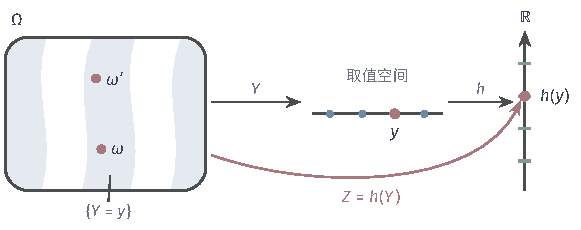
\includegraphics[width=98mm]{figures/07-probability/02-measure-theoretic-probability/tikz/cexp-factorization/figure.pdf}
  \caption{经由观测的因子分解。左边$\Omega$被分成水平集$\{Y=y\}$（浅蓝与白色条带）；同一条带内的$\omega$与$\omega'$有相同的$Y$值，因而$\sigma(Y)$可测的$Z$在两点取值相同。于是$Z$可以先经$Y$映到取值空间，再经可测函数$h$映到$\mathbb{R}$，即$Z=h(Y)$。}
  \label{fig:cexp-factorization}
\end{BookInlineFigure}

\begin{lemma}[因子分解引理]
\label{lem:cexp-factorization}
设$Y:\Omega\to E$关于$\mathcal{E}$可测，$Z:\Omega\to\mathbb{R}$关于$\sigma(Y)$可测。则存在可测函数$h:E\to\mathbb{R}$，使$Z=h(Y)$在$\Omega$上处处成立。
\end{lemma}

\begin{proof}
先设$Z$是示性函数$\mathbf{1}_{A}$，$A\in\sigma(Y)$。由$\sigma(Y)$的定义，有$B\in\mathcal{E}$使$A=\{Y\in B\}$，于是
\[
 Z=\mathbf{1}_{B}(Y),
\]
取$h=\mathbf{1}_{B}$即可。若$Z$是有限个这样的示性函数的线性组合$\sum_{i}a_i\mathbf{1}_{A_i}$，对每个$A_i$取对应的$B_i$，令$h=\sum_ia_i\mathbf{1}_{B_i}$。

一般情形，取$\sigma(Y)$可测的简单函数$Z_n$，使$Z_n(\omega)\to Z(\omega)$对每个$\omega$成立；例如把$\max(-n,\min(Z,n))$向零截断到$2^{-n}$的整数倍。由上一段，$Z_n=h_n(Y)$，$h_n$可测。令
\[
 L=\bigl\{e\in E:\ \lim_{n\to\infty}h_n(e)\ \text{存在且有限}\bigr\},
\]
它是$\limsup_nh_n$与$\liminf_nh_n$相等且有限的点集，因而可测；在$L$上令$h=\lim_nh_n$，在$L$外令$h=0$，$h$可测。对每个$\omega$，数列$h_n(Y(\omega))=Z_n(\omega)$收敛到$Z(\omega)$，所以$Y(\omega)\in L$，并且$h(Y(\omega))=Z(\omega)$。
\end{proof}

把引理用于$\mathbb{E}[X\mid Y]$的任一版本，得到可测函数$m:E\to\mathbb{R}$，使
\begin{equation}
 \mathbb{E}[X\mid Y]=m(Y).
 \label{eq:cexp-regression-function}
\end{equation}
按惯例记$\mathbb{E}[X\mid Y=y]=m(y)$。由于$\sigma(Y)$中的事件都是$\{Y\in B\}$，并且$\mathbb{E}[m(Y)\mathbf{1}_B(Y)]$可以用推前分布写成对$P_Y$的积分，一个可测函数$m$满足要求，当且仅当$m(Y)$可积，并且对每个$B\in\mathcal{E}$，
\begin{equation}
 \mathbb{E}\bigl[X\mathbf{1}_{\{Y\in B\}}\bigr]=\int_{B}m(y)\,P_Y(\mathrm{d}y).
 \label{eq:cexp-given-variable-check}
\end{equation}

\paragraph{函数只在分布下几乎处处确定}
$m(Y)$与$m(y)$要分清。前者是$\Omega$上的随机变量，作为条件期望的版本，几乎必然唯一；后者是取值空间上的普通函数。两个函数$m,\tilde m$都满足要求，当且仅当$m(Y)=\tilde m(Y)$几乎必然成立，也就是
\[
 P_Y\bigl(\{y:\ m(y)\neq\tilde m(y)\}\bigr)=\mathbb{P}\bigl(m(Y)\neq\tilde m(Y)\bigr)=0 .
\]
所以$m$只在$P_Y$几乎处处的意义下确定：在$Y$取不到的地方，$m$可以任意取值；在$Y$以零概率取到的单个点上，$m$的值也没有意义。

“只知绝对值”的例子把这一点画得很清楚。$Y=\lvert X\rvert\sim\operatorname{Unif}(0,1)$，$m(y)=y/2$是$\mathbb{E}[X^{+}\mid Y=y]$的一个版本。把$m$在$y=1/2$处改成$0.9$，并在$[0,1]$之外任意改动，得到的$\tilde m$仍是一个版本，见图~\ref{fig:cexp-versions}(a)。在$\Omega$上看，$\tilde m(Y)$与$m(Y)$只在$\omega=\pm1/2$两点不同，见图~\ref{fig:cexp-versions}(b)。问“已知$\lvert X\rvert=1/2$时$X^{+}$的平均是多少”，单凭条件期望的定义无法回答；要给单个观测值指定确定的条件平均，需要额外的要求，例如$m$的连续性，这在第~\ref{chap:conditional-distributions}章讨论。

\begin{BookInlineFigure}
  \centering
  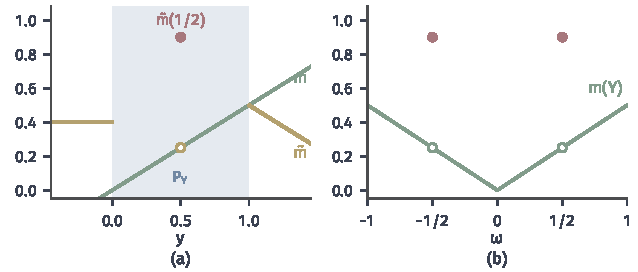
\includegraphics[width=108mm]{figures/07-probability/02-measure-theoretic-probability/matplotlib/cexp-versions/figure.pdf}
  \caption{$\mathbb{E}[X^{+}\mid Y]$的两个版本，$Y=\lvert X\rvert$，$X\sim\operatorname{Unif}(-1,1)$。(a)绿线$m(y)=y/2$；黄线与红点组成的$\tilde m$在$[0,1]$上只在$y=1/2$处不同，在浅蓝区间$[0,1]$（$P_Y$所在之处）以外任意取值。(b)复合到$\Omega$上，$\tilde m(Y)$与$m(Y)$只在$\omega=\pm1/2$两点（红点）不同。}
  \label{fig:cexp-versions}
\end{BookInlineFigure}

\paragraph{回到条件均值的公式}
式~\eqref{eq:cexp-given-variable-check}说明，第~\ref{chap:random-vectors}章的两个公式都给出了版本。若$Y$只取可数多个值，对$\mathbb{P}(Y=y)>0$的$y$令
\[
 m(y)=\frac{\mathbb{E}\bigl[X\mathbf{1}_{\{Y=y\}}\bigr]}{\mathbb{P}(Y=y)},
\]
其余$y$上任意取值。两边对$B$中的$y$求和，式~\eqref{eq:cexp-given-variable-check}成立，交换求和与期望由$\mathbb{E}\lvert X\rvert<\infty$保证。

若$(X,Y)$有联合密度$f_{X,Y}$，$Y$为实值，在$f_Y(y)>0$处令
\[
 m(y)=\frac{1}{f_Y(y)}\int x\,f_{X,Y}(x,y)\,\mathrm{d}x ,
\]
其余$y$上令$m(y)=0$。由$\mathbb{E}\lvert X\rvert<\infty$与Fubini定理，
\[
 \mathbb{E}\bigl[X\mathbf{1}_{\{Y\in B\}}\bigr]=\int_{B}\int x\,f_{X,Y}(x,y)\,\mathrm{d}x\,\mathrm{d}y=\int_{B}m(y)f_Y(y)\,\mathrm{d}y ,
\]
这正是式~\eqref{eq:cexp-given-variable-check}。$f_Y(y)=0$的那些$y$对右边没有贡献，$m$在那里怎样取都可以。

没有密度时，可以像前面那样直接验证候选。在“只知绝对值”的例子中，对满足$\mathbb{E}\lvert g(X)\rvert<\infty$的可测函数$g$，把积分按$\pm x$配对，
\[
 \mathbb{E}\bigl[g(X)\mathbf{1}_{\{Y\in B\}}\bigr]
 =\int_{0}^{1}\frac{g(y)+g(-y)}{2}\,\mathbf{1}_{B}(y)\,\mathrm{d}y .
\]
右边正是式~\eqref{eq:cexp-given-variable-check}，其中$P_Y$是$[0,1]$上的均匀分布，所以
\begin{equation}
 \mathbb{E}\bigl[g(X)\bigm|\lvert X\rvert\bigr]=\frac{g(\lvert X\rvert)+g(-\lvert X\rvert)}{2}.
 \label{eq:cexp-folding}
\end{equation}
取$g(x)=x^{+}$得到$\lvert X\rvert/2$；取$g(x)=x$得到$0$；取$g(x)=\mathrm{e}^{x}$得到$\cosh\lvert X\rvert$，见图~\ref{fig:cexp-folding}(b)。


\section{基本性质}
\label{sec:cexp-properties}

有了定义，下一步是学会运算。在有限分组中，组内平均对随机变量是线性的、保序的，已经知道的量在组内是常数，可以提到平均号外面。这些性质在一般的$\mathcal{G}$下是否仍然成立？本节固定信息$\mathcal{G}$，逐条从积分定义核验它们，并用传感器表检验计算含义。核验的办法都相同：写出候选，检查它$\mathcal{G}$可测、可积，并在每个$A\in\mathcal{G}$上满足式~\eqref{eq:cexp-defining}，再由定理~\ref{thm:cexp-existence}的唯一性得出几乎必然相等。最后讨论另一种极端：当信息与变量独立时，条件平均就是普通的平均。

\subsection{线性与保序}
\label{sec:cexp-linearity}

先看两条最基本的规则。在每一组内求平均，和的平均是平均的和，较大变量的平均不小于较小变量的平均。下面的定理说明它们对一般信息仍然成立，只是相等与不等都按几乎必然理解。

\begin{theorem}[线性与保序]
\label{thm:cexp-linearity}
设$X_1,X_2$可积，$a,b$是实数。则
\begin{equation}
 \mathbb{E}[aX_1+bX_2\mid\mathcal{G}]=a\,\mathbb{E}[X_1\mid\mathcal{G}]+b\,\mathbb{E}[X_2\mid\mathcal{G}].
 \label{eq:cexp-linearity}
\end{equation}
若$X_1\leq X_2$几乎必然成立，则
\begin{equation}
 \mathbb{E}[X_1\mid\mathcal{G}]\leq\mathbb{E}[X_2\mid\mathcal{G}].
 \label{eq:cexp-monotone}
\end{equation}
特别地，常数$c$满足$\mathbb{E}[c\mid\mathcal{G}]=c$，并且
\begin{equation}
 \bigl\lvert\mathbb{E}[X_1\mid\mathcal{G}]\bigr\rvert\leq\mathbb{E}\bigl[\lvert X_1\rvert\bigm|\mathcal{G}\bigr].
 \label{eq:cexp-abs}
\end{equation}
\end{theorem}

\begin{proof}
记$Z_1,Z_2$为$X_1,X_2$的条件期望的版本。

\emph{线性。}$aZ_1+bZ_2$是$\mathcal{G}$可测的可积函数。对$A\in\mathcal{G}$，由期望的线性和式~\eqref{eq:cexp-defining}，
\[
 \mathbb{E}\bigl[(aZ_1+bZ_2)\mathbf{1}_{A}\bigr]
 =a\,\mathbb{E}[X_1\mathbf{1}_{A}]+b\,\mathbb{E}[X_2\mathbf{1}_{A}]
 =\mathbb{E}\bigl[(aX_1+bX_2)\mathbf{1}_{A}\bigr].
\]
所以$aZ_1+bZ_2$是$aX_1+bX_2$的条件期望的一个版本，由唯一性得式~\eqref{eq:cexp-linearity}。

\emph{非负性。}先设$X\geq0$几乎必然成立，$Z$是$\mathbb{E}[X\mid\mathcal{G}]$的版本。事件$A=\{Z<0\}$属于$\mathcal{G}$，于是
\[
 \mathbb{E}[Z\mathbf{1}_{A}]=\mathbb{E}[X\mathbf{1}_{A}]\geq0 .
\]
另一方面$Z\mathbf{1}_{A}\leq0$，期望不大于零。两者合起来，$Z\mathbf{1}_{A}$是期望为零的非正函数，几乎必然为零；它在$A$上严格为负，所以$\mathbb{P}(A)=0$，即$Z\geq0$几乎必然成立。

\emph{保序。}对$X_2-X_1\geq0$用非负性，再用线性，得式~\eqref{eq:cexp-monotone}。由$-\lvert X_1\rvert\leq X_1\leq\lvert X_1\rvert$与保序，得到绝对值的不等式。常数$c$本身是$\mathcal{G}$可测的，满足定义的三条要求。
\end{proof}

线性对应于“组内平均可以逐项计算”，保序对应于“逐点更大的量，组内平均也更大”。在传感器表上，$\mathbb{E}[2Y-1\mid X]=2\,\mathbb{E}[Y\mid X]-1$，三行依次是
\[
 2\cdot\tfrac13-1=-\tfrac13,\qquad 2\cdot1-1=1,\qquad 2\cdot\tfrac53-1=\tfrac73 ,
\]
与直接按行求$2Y-1$的平均相同。又因为$0\leq Y\leq2$，保序给出$0\leq\mathbb{E}[Y\mid X]\leq2$，三个行均值确实落在这个范围。

“几乎必然”在这里有一个实际后果。式~\eqref{eq:cexp-linearity}对每一对$(X_1,X_2)$和每一对系数，都在一个可能依赖于它们的零概率集之外成立。对可数多个这样的等式，把例外集并起来仍是零概率集，可以同时使用；对不可数多个，例如对所有实数$a$同时成立，就不能直接合并例外集。逐事件的条件概率要拼成一个完整的分布，正卡在这一点上，第~\ref{chap:conditional-distributions}章会处理它。

\subsection{提取已知量}
\label{sec:cexp-known}

\paragraph{已知的乘子可以提出}
在一组之内，$\mathcal{G}$可测的量是常数，常数可以从平均里提出来。传感器表中，给定$X$时$X$已知，所以应当有$\mathbb{E}[XY\mid X]=X\,\mathbb{E}[Y\mid X]$。这条规则称为\term{提取已知量}（taking out what is known）。下面的定理说明它对一般信息成立，并说明乘子需要满足什么条件。

\begin{theorem}[提取已知量]
\label{thm:cexp-known}
设$H$是$\mathcal{G}$可测的随机变量，$X$与$HX$都可积。则$H\,\mathbb{E}[X\mid\mathcal{G}]$可积，并且
\begin{equation}
 \mathbb{E}[HX\mid\mathcal{G}]=H\,\mathbb{E}[X\mid\mathcal{G}].
 \label{eq:cexp-known}
\end{equation}
特别地，若$H$是$\mathcal{G}$可测且可积的，则$\mathbb{E}[H\mid\mathcal{G}]=H$。
\end{theorem}

证明分三步扩大乘子的范围：先是示性函数，再是有界函数，最后是一般函数。前两步是定义的直接推论；最后一步的难点在于，事先并不知道$HZ$可积，不能直接用控制收敛定理，需要先对非负的情形用单调收敛定理得到可积性。

\begin{proof}
记$Z=\mathbb{E}[X\mid\mathcal{G}]$。$HZ$是两个$\mathcal{G}$可测函数之积，本身$\mathcal{G}$可测。由唯一性，只需证明$HZ$可积，并且对每个$A\in\mathcal{G}$，
\[
 \mathbb{E}[HX\mathbf{1}_{A}]=\mathbb{E}[HZ\mathbf{1}_{A}] .
\]

\emph{第一步，示性函数与简单函数。}设$H=\mathbf{1}_{B}$，$B\in\mathcal{G}$。$A\cap B\in\mathcal{G}$，由式~\eqref{eq:cexp-defining}，
\[
 \mathbb{E}[\mathbf{1}_{B}X\mathbf{1}_{A}]=\mathbb{E}[X\mathbf{1}_{A\cap B}]=\mathbb{E}[Z\mathbf{1}_{A\cap B}]=\mathbb{E}[\mathbf{1}_{B}Z\mathbf{1}_{A}] .
\]
由线性，结论对$\mathcal{G}$可测的简单函数$H$成立。

\emph{第二步，有界的$H$。}设$\lvert H\rvert\leq c$。取$\mathcal{G}$可测的简单函数$H_n$，使$\lvert H_n\rvert\leq c$且$H_n\to H$逐点成立。由第一步，
\[
 \mathbb{E}[H_nX\mathbf{1}_{A}]=\mathbb{E}[H_nZ\mathbf{1}_{A}] .
\]
左边被积函数被$c\lvert X\rvert$控制，右边被$c\lvert Z\rvert$控制，两者都可积。由控制收敛定理令$n\to\infty$，两边分别趋于$\mathbb{E}[HX\mathbf{1}_{A}]$与$\mathbb{E}[HZ\mathbf{1}_{A}]$。

\emph{第三步，非负的$H$与$X$。}设$H\geq0$，$X\geq0$，于是$Z\geq0$。令$H_n=\min(H,n)$，由第二步，
\[
 \mathbb{E}[H_nX\mathbf{1}_{A}]=\mathbb{E}[H_nZ\mathbf{1}_{A}] .
\]
两边的被积函数都非负并且随$n$单调增加，由单调收敛定理令$n\to\infty$，得到
\[
 \mathbb{E}[HX\mathbf{1}_{A}]=\mathbb{E}[HZ\mathbf{1}_{A}] .
\]
取$A=\Omega$，左边是有限的$\mathbb{E}[HX]$，所以$HZ$可积。

\emph{第四步，一般情形。}写$H=H^{+}-H^{-}$，$X=X^{+}-X^{-}$，并记$Z_{\pm}=\mathbb{E}[X^{\pm}\mid\mathcal{G}]$，于是$Z=Z_{+}-Z_{-}$。四个乘积$H^{\pm}X^{\pm}$都被$\lvert HX\rvert$控制，因而可积。对每一对符号用第三步，得到$H^{\pm}Z_{\pm}$可积，且
\[
 \mathbb{E}[H^{\pm}X^{\pm}\mathbf{1}_{A}]=\mathbb{E}[H^{\pm}Z_{\pm}\mathbf{1}_{A}] .
\]
把四个等式按$HX=(H^{+}-H^{-})(X^{+}-X^{-})$的符号相加，右边合成$\mathbb{E}[HZ\mathbf{1}_{A}]$，左边合成$\mathbb{E}[HX\mathbf{1}_{A}]$；而$\lvert HZ\rvert$不超过四个可积函数$H^{\pm}Z_{\pm}$之和，所以$HZ$可积。

最后一句取$X=1$：$\mathbb{E}[1\mid\mathcal{G}]=1$，$H\cdot1$可积，于是$\mathbb{E}[H\mid\mathcal{G}]=H$。
\end{proof}

定理要求$HX$可积，否则左边的条件期望在本章的意义下没有定义。乘子本身不必有界：$X$与$HX$可积就够了，结论里$H\,\mathbb{E}[X\mid\mathcal{G}]$的可积性是证明出来的，不是假设的。

\paragraph{传感器表上的计算}
在传感器表中取$H=X$，它是$\sigma(X)$可测的。由式~\eqref{eq:cexp-known}与三行的条件均值，
\[
 \mathbb{E}[XY\mid X]=X\,\mathbb{E}[Y\mid X]:\qquad 0\cdot\tfrac13=0,\qquad 1\cdot1=1,\qquad 2\cdot\tfrac53=\tfrac{10}{3},
\]
见图~\ref{fig:cexp-known-factor}(a)。直接计算第三行核对：第三行中$Y$以条件概率$\tfrac13,\tfrac23$取$1,2$，$XY$取$2,4$，平均为$\tfrac23+\tfrac83=\tfrac{10}{3}$。

\begin{BookInlineFigure}
  \centering
  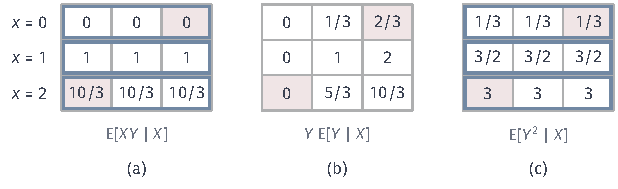
\includegraphics[width=104mm]{figures/07-probability/02-measure-theoretic-probability/tikz/cexp-known-factor/figure.pdf}
  \caption{提取已知量，传感器表，浅红格的概率为零。(a)$\mathbb{E}[XY\mid X]=X\,\mathbb{E}[Y\mid X]$，每行取常数$0$、$1$、$10/3$（蓝框表示行内为常数）。(b)$Y\,\mathbb{E}[Y\mid X]$在同一行内变化，不是$X$的函数。(c)$\mathbb{E}[Y^{2}\mid X]$，每行取$1/3$、$3/2$、$3$。}
  \label{fig:cexp-known-factor}
\end{BookInlineFigure}

\paragraph{未知的乘子不能提出}
乘子必须是已知的。若把$Y$当作乘子，“$\mathbb{E}[Y\cdot Y\mid X]=Y\,\mathbb{E}[Y\mid X]$”就是错的。右边在同一行内随$Y$变化，见图~\ref{fig:cexp-known-factor}(b)，它不是$\sigma(X)$可测的，根本不可能是给定$X$的条件期望。正确的值由行内平均给出：
\[
 \mathbb{E}[Y^{2}\mid X=0]=\tfrac13,\qquad \mathbb{E}[Y^{2}\mid X=1]=\tfrac32,\qquad \mathbb{E}[Y^{2}\mid X=2]=3 ,
\]
见图~\ref{fig:cexp-known-factor}(c)。例如第二行中$Y^{2}$以$\tfrac14,\tfrac12,\tfrac14$取$0,1,4$，平均为$\tfrac12+1=\tfrac32$。在组内，已知量是常数，未知量仍在变化；只有前者能提到平均号外面。

\subsection{独立情形}
\label{sec:cexp-independence}

\paragraph{与信息独立的变量}
如果已知的信息与$X$毫无关联，给定这份信息的平均就不应改变。称$X$与$\mathcal{G}$独立，是指对每个Borel集$B$与每个$A\in\mathcal{G}$，事件$\{X\in B\}$与$A$独立，也就是$\sigma(X)$与$\mathcal{G}$独立。这时$X$与每个$\mathbf{1}_{A}$是独立的随机变量，由第~\ref{chap:probability-spaces}章的积分表示，两个独立可积变量乘积的期望等于期望的乘积。

\begin{theorem}[独立的信息]
\label{thm:cexp-independent}
设$X$可积并且与$\mathcal{G}$独立。则
\begin{equation}
 \mathbb{E}[X\mid\mathcal{G}]=\mathbb{E}[X].
 \label{eq:cexp-independent}
\end{equation}
\end{theorem}

\begin{proof}
常数$\mathbb{E}[X]$是$\mathcal{G}$可测且可积的。对$A\in\mathcal{G}$，$X$与$\mathbf{1}_{A}$独立且都可积，乘积的期望等于期望的乘积，
\[
 \mathbb{E}[X\mathbf{1}_{A}]=\mathbb{E}[X]\,\mathbb{P}(A)=\mathbb{E}\bigl[\mathbb{E}[X]\,\mathbf{1}_{A}\bigr].
\]
所以常数$\mathbb{E}[X]$满足式~\eqref{eq:cexp-defining}。
\end{proof}

“只知绝对值”的例子提供了一个独立的情形。记$S=\operatorname{sgn}X$，它以各$\tfrac12$的概率取$\pm1$。对$0\leq t\leq1$，
\[
 \mathbb{P}\bigl(S=1,\ \lvert X\rvert\leq t\bigr)=\mathbb{P}(0<X\leq t)=\frac t2=\mathbb{P}(S=1)\,\mathbb{P}\bigl(\lvert X\rvert\leq t\bigr),
\]
所以符号与绝对值独立。由定理~\ref{thm:cexp-independent}，$\mathbb{E}[S\mid\lvert X\rvert]=\mathbb{E}[S]=0$：知道离原点多远，对“在哪一侧”毫无帮助。再由$X=S\lvert X\rvert$与提取已知量，
\[
 \mathbb{E}\bigl[X\bigm|\lvert X\rvert\bigr]=\lvert X\rvert\,\mathbb{E}\bigl[S\bigm|\lvert X\rvert\bigr]=0 ,
\]
与式~\eqref{eq:cexp-folding}取$g(x)=x$的结果一致。

\paragraph{条件平均为常数不能推出独立}
定理~\ref{thm:cexp-independent}的逆命题不成立。上面刚得到$\mathbb{E}[X\mid\lvert X\rvert]=0=\mathbb{E}[X]$，可是$X$与$\lvert X\rvert$不独立，取一对事件就能看出：
\[
 \mathbb{P}\bigl(\lvert X\rvert\leq\tfrac12,\ X>\tfrac12\bigr)=0,\qquad
 \mathbb{P}\bigl(\lvert X\rvert\leq\tfrac12\bigr)\,\mathbb{P}\bigl(X>\tfrac12\bigr)=\tfrac12\cdot\tfrac14=\tfrac18 .
\]
图~\ref{fig:cexp-independence}比较了两种情形。左边给定$\lvert X\rvert=y$后，$X$只能是$\pm y$，条件规律随$y$剧烈变化，只是两点的平均恰好总为$0$；右边$Z$与$X$独立，给定$Z$后$X$的整个分布都不变。两者的条件平均都是常数$0$，图中的红线完全相同。

\begin{BookInlineFigure}
  \centering
  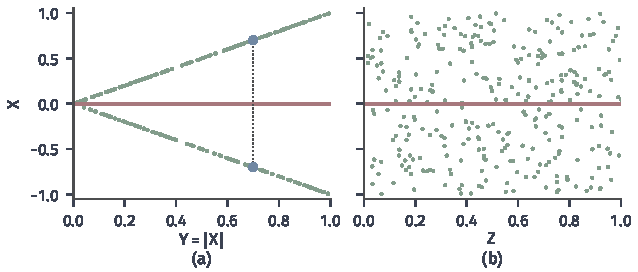
\includegraphics[width=108mm]{figures/07-probability/02-measure-theoretic-probability/matplotlib/cexp-independence/figure.pdf}
  \caption{条件平均为常数不等于独立。随机数种子$7$，各$300$个模拟点（绿）。(a)$X\sim\operatorname{Unif}(-1,1)$与$Y=\lvert X\rvert$，点落在两条线段$x=\pm y$上；给定$Y=0.7$时$X$只取蓝点$\pm0.7$，条件平均为$0$（红线）。(b)$X\sim\operatorname{Unif}(-1,1)$与独立的$Z\sim\operatorname{Unif}(0,1)$，点铺满矩形，条件平均同样为$0$。}
  \label{fig:cexp-independence}
\end{BookInlineFigure}

条件平均为常数只约束一个数：每组的平均都等于总平均。独立则要求给定信息后$X$落在任何集合中的条件概率都不变，即对一切Borel集$B$，
\[
 \mathbb{E}\bigl[\mathbf{1}_{\{X\in B\}}\bigm|\mathcal{G}\bigr]=\mathbb{P}(X\in B).
\]
前者只要求$X$本身的条件平均不变，后者要求每个示性函数$\mathbf{1}_{\{X\in B\}}$的条件平均都不变，由后者可以推出前者。给定信息后完整的条件规律在第~\ref{chap:conditional-distributions}章研究，那里的条件独立也要求整个条件分布满足乘积关系，而不只是条件均值。


\section{迭代条件期望}
\label{sec:cexp-iterated}

条件期望$\mathbb{E}[X\mid\mathcal{G}]$本身是一个可积的随机变量，可以再对它求期望，或者再给定另一份信息求条件期望。这样平均两次，结果是什么？分两种情况：一种是第二次什么也不给定，条件被完全取消；另一种是第二次保留另一层信息。后一种情况能否化简，取决于两份信息之间有没有包含关系。

\subsection{全期望公式}
\label{sec:cexp-total-expectation}

\paragraph{先分组平均，再按组加权}
取消条件的情形最简单：在式~\eqref{eq:cexp-defining}中取$A=\Omega$。$\Omega$总在$\mathcal{G}$中，于是得到下面的定理。

\begin{theorem}[全期望公式]
\label{thm:cexp-total-expectation}
设$X$可积，$\mathcal{G}\subseteq\mathcal{F}$是$\sigma$代数。则
\begin{equation}
 \mathbb{E}\bigl[\mathbb{E}[X\mid\mathcal{G}]\bigr]=\mathbb{E}[X].
 \label{eq:cexp-total-expectation}
\end{equation}
\end{theorem}

\begin{proof}
在式~\eqref{eq:cexp-defining}中取$A=\Omega$，$\mathbf{1}_{\Omega}=1$。
\end{proof}

证明只有一行，含义却很具体。在有限划分中，$\mathbb{E}[X\mid\mathcal{G}]$在第$i$组取$c_i$，所以它的期望是$\sum_ic_i\mathbb{P}(A_i)$：先在每一组内求平均，再以各组的概率为权重把组平均加起来，就恢复了总平均。把概率看成质量，这就是“整体的重心等于各部分重心按质量加权的重心”。

传感器表上的计算见图~\ref{fig:cexp-total-expectation}。三行的质量依次是$0.3,0.4,0.3$，行内重心是$1/3,1,5/3$；把每行的质量集中到它的重心，再求这三个点的重心，
\[
 0.3\cdot\tfrac13+0.4\cdot1+0.3\cdot\tfrac53=0.1+0.4+0.5=1=\mathbb{E}[Y].
\]

\begin{BookInlineFigure}
  \centering
  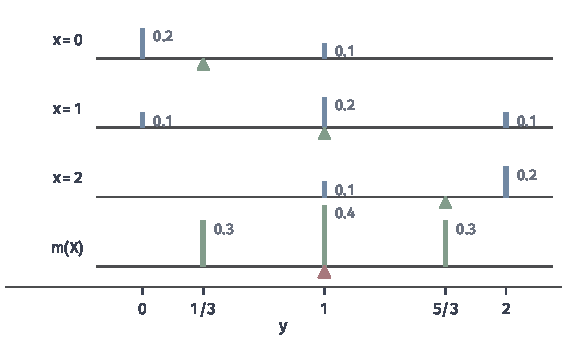
\includegraphics[width=96mm]{figures/07-probability/02-measure-theoretic-probability/matplotlib/cexp-total-expectation/figure.pdf}
  \caption{全期望公式是重心的合成，传感器表。上面三层是三行中的联合质量（蓝色竖线，高度与质量成正比），绿色三角是各行的重心$1/3$、$1$、$5/3$。最下一层把各行的质量$0.3$、$0.4$、$0.3$移到行重心（绿色竖线），它们的重心是$\mathbb{E}[Y]=1$（红色三角）。}
  \label{fig:cexp-total-expectation}
\end{BookInlineFigure}

逐次等分的例子同样可以核对。$\mathcal{G}_2$的四段各占$1/4$，段内平均是$\tfrac{1}{48},\tfrac{7}{48},\tfrac{19}{48},\tfrac{37}{48}$，于是
\[
 \mathbb{E}\bigl[\mathbb{E}[X\mid\mathcal{G}_2]\bigr]=\frac14\cdot\frac{1+7+19+37}{48}=\frac{64}{192}=\frac13=\int_0^1\omega^{2}\,\mathrm{d}\omega .
\]

\paragraph{统一求和与积分}
第~\ref{chap:random-vectors}章分别对概率表和联合密度证明了全期望公式，现在两者都是式~\eqref{eq:cexp-total-expectation}的特例。给定观测$Y$时，$\mathbb{E}[X\mid Y]=m(Y)$，由推前分布的积分公式，
\[
 \mathbb{E}[X]=\mathbb{E}\bigl[m(Y)\bigr]=\int m(y)\,P_Y(\mathrm{d}y).
\]
$Y$只取可数多个值时，右边是$\sum_ym(y)\,p_Y(y)$；$Y$有密度时，右边是$\int m(y)f_Y(y)\,\mathrm{d}y$。两种计算方式只是对$P_Y$积分的两种具体写法。

全期望公式在没有密度时同样好用。“只知绝对值”的例子中，由式~\eqref{eq:cexp-folding}，$\mathrm{e}^{X}$给定$\lvert X\rvert$的条件期望是$\cosh\lvert X\rvert$，而$\lvert X\rvert\sim\operatorname{Unif}(0,1)$，于是
\[
 \mathbb{E}[\mathrm{e}^{X}]=\mathbb{E}\bigl[\cosh\lvert X\rvert\bigr]=\int_0^1\cosh y\,\mathrm{d}y=\sinh 1 .
\]
直接计算得到同样的结果：
\[
 \mathbb{E}[\mathrm{e}^{X}]=\frac12\int_{-1}^{1}\mathrm{e}^{x}\,\mathrm{d}x=\frac{\mathrm{e}-\mathrm{e}^{-1}}{2}=\sinh1 .
\]
先把对称的两点合并，被积函数变成偶函数$\cosh$，积分区间减半；这正是先分组平均、再对组求平均的计算方式。

\subsection{塔式法则}
\label{sec:cexp-tower}

\paragraph{嵌套的信息}
现在第二次平均也保留一些信息。设$\mathcal{H}\subseteq\mathcal{G}$：$\mathcal{H}$中的事件都能由$\mathcal{G}$判断，$\mathcal{H}$是较少的信息。有限划分时，这表示$\mathcal{H}$的每一组都是$\mathcal{G}$的若干组之并，即$\mathcal{G}$是$\mathcal{H}$的细分。

传感器表中取$\mathcal{G}=\sigma(X)$，再取$\mathcal{H}=\sigma(\mathbf{1}_{\{X=2\}})$，后者只知道第一台“是否读偏高”，把前两行并成一组$\{X\leq1\}$，第三行单独一组。先按行平均，再在$\mathcal{H}$的组内平均：$\{X\leq1\}$的概率是$0.7$，其中前两行的质量分别是$0.3$与$0.4$，于是
\[
 \mathbb{E}\bigl[\mathbb{E}[Y\mid X]\bigm|\mathcal{H}\bigr]=\frac{0.3\cdot\frac13+0.4\cdot1}{0.7}=\frac{0.5}{0.7}=\frac57\quad\text{在}\ \{X\leq1\}\ \text{上}.
\]
另一方面，直接在$\{X\leq1\}$上求$Y$的平均，五个正概率格子上的累计期望是$0.1+0.4=0.5$，同样得$5/7$。第三行在两种算法下都是$5/3$。图~\ref{fig:cexp-tower-nested}画出了这两条路径。

\begin{BookInlineFigure}
  \centering
  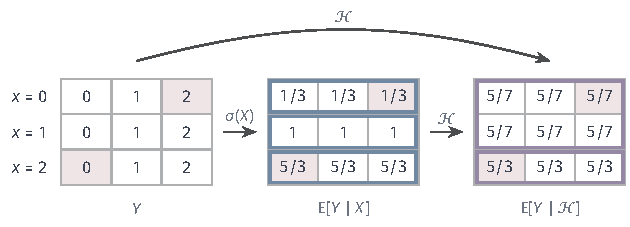
\includegraphics[width=106mm]{figures/07-probability/02-measure-theoretic-probability/tikz/cexp-tower-nested/figure.pdf}
  \caption{嵌套信息下的塔式法则，传感器表，浅红格概率为零。左：$Y$在九个格子上的值。中：$\mathbb{E}[Y\mid X]$，在每行（蓝框）取常数。右：$\mathbb{E}[Y\mid\mathcal{H}]$，$\mathcal{H}=\sigma(\mathbf{1}_{\{X=2\}})$的两组（紫框）上分别取$5/7$与$5/3$。下方两步与上方一步得到相同的结果。}
  \label{fig:cexp-tower-nested}
\end{BookInlineFigure}

\paragraph{先细后粗与先粗后细}
两种顺序都得到较粗信息上的条件期望。

\begin{theorem}[塔式法则]
\label{thm:cexp-tower}
设$X$可积，$\mathcal{H}\subseteq\mathcal{G}\subseteq\mathcal{F}$都是$\sigma$代数。则
\begin{equation}
 \mathbb{E}\bigl[\mathbb{E}[X\mid\mathcal{G}]\bigm|\mathcal{H}\bigr]=\mathbb{E}[X\mid\mathcal{H}]
 =\mathbb{E}\bigl[\mathbb{E}[X\mid\mathcal{H}]\bigm|\mathcal{G}\bigr].
 \label{eq:cexp-tower}
\end{equation}
\end{theorem}

\begin{proof}
\emph{先细后粗。}记$Z=\mathbb{E}[X\mid\mathcal{G}]$，它可积。要证$\mathbb{E}[X\mid\mathcal{H}]$是$\mathbb{E}[Z\mid\mathcal{H}]$的一个版本。它是$\mathcal{H}$可测且可积的；对$A\in\mathcal{H}$，因为$\mathcal{H}\subseteq\mathcal{G}$，$A$也在$\mathcal{G}$中，两次使用式~\eqref{eq:cexp-defining}，
\[
 \mathbb{E}[Z\mathbf{1}_{A}]=\mathbb{E}[X\mathbf{1}_{A}]=\mathbb{E}\bigl[\mathbb{E}[X\mid\mathcal{H}]\,\mathbf{1}_{A}\bigr].
\]
第一个等号用了$A\in\mathcal{G}$，第二个等号用了$A\in\mathcal{H}$。

\emph{先粗后细。}$\mathbb{E}[X\mid\mathcal{H}]$是$\mathcal{H}$可测的，因而也是$\mathcal{G}$可测的，并且可积。由定理~\ref{thm:cexp-known}的最后一句，给定$\mathcal{G}$对它求条件期望，结果是它自身。
\end{proof}

式~\eqref{eq:cexp-tower}称为\term{塔式法则}（tower property）。两个等号的来源不同。先细后粗用的是积分定义：较粗信息下的已知事件，在较细信息下也是已知的，累计期望在两层平均中都被保留。先粗后细用的是“已知量不变”：粗信息下的平均在细信息下已经是已知量，再平均也不改变。两者合起来，迭代的结果总是较粗的那一层，较少的信息胜出。全期望公式是$\mathcal{H}=\{\emptyset,\Omega\}$的特例。

\paragraph{没有包含关系时}
塔式法则依赖$\mathcal{H}\subseteq\mathcal{G}$。两份信息互不包含时，迭代的顺序会影响结果，也不能换成在两者共有的信息上求平均。仍用传感器表，取$\sigma(X)$（按行分组）与$\sigma(D)$（按对角线分组，$D=X-Y$）。

先按行平均，再按对角线平均。$\mathbb{E}[Y\mid X]$在$D=1$的两格$(1,0)$与$(2,1)$上分别取$1$与$5/3$，两格概率相等，于是在$\{D=1\}$上
\[
 \mathbb{E}\bigl[\mathbb{E}[Y\mid X]\bigm|D\bigr]=\frac12\Bigl(1+\frac53\Bigr)=\frac43 .
\]
同样算得$\{D=0\}$上为$1$，$\{D=-1\}$上为$2/3$，见图~\ref{fig:cexp-tower-non-nested}(a)。

反过来，先按对角线平均，再按行平均。$\mathbb{E}[Y\mid D]$在第一行的两个正概率格子$(0,0)$与$(0,1)$上分别取$1$与$3/2$，两格概率为$0.2$与$0.1$，于是在$\{X=0\}$上
\[
 \mathbb{E}\bigl[\mathbb{E}[Y\mid D]\bigm|X\bigr]=\frac{0.2\cdot1+0.1\cdot\frac32}{0.3}=\frac76 .
\]
另外两行分别得到$1$与$5/6$，见图~\ref{fig:cexp-tower-non-nested}(b)。

\begin{BookInlineFigure}
  \centering
  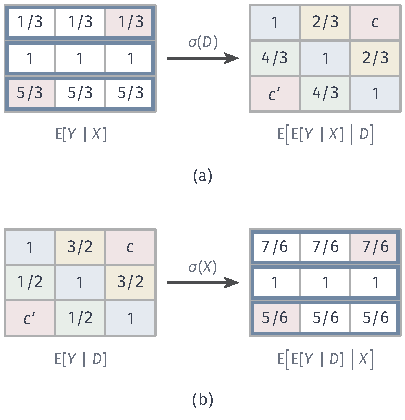
\includegraphics[width=68mm]{figures/07-probability/02-measure-theoretic-probability/tikz/cexp-tower-non-nested/figure.pdf}
  \caption{互不包含的两份信息，传感器表。蓝框表示按行（$\sigma(X)$）取常数，同色格子表示按对角线（$\sigma(D)$，$D=X-Y$）取常数，$c$、$c'$是零概率组上的任意常数。(a)先给定$X$再给定$D$。(b)先给定$D$再给定$X$。两个结果不同，也都不是常数$\mathbb{E}[Y]=1$。}
  \label{fig:cexp-tower-non-nested}
\end{BookInlineFigure}

两种顺序的结果一个是$D$的函数，一个是$X$的函数，彼此不同。它们也都不等于在共同信息$\sigma(X)\cap\sigma(D)$上的平均：一个事件若同时是若干整行之并和若干整条对角线之并，只要含有某一行，就含有这一行经过的对角线，进而含有那些对角线经过的其他行，最后只能是$\Omega$；所以共同信息只有$\{\emptyset,\Omega\}$，相应的平均是常数$1$。两份信息各自有用，交起来却什么也不剩，先后两次平均在两种顺序下也都没有抵达这个常数。


\section{条件期望的不等式}
\label{sec:cexp-inequalities}

条件期望对线性运算可以逐项进行，对非线性运算却不行：$\mathbb{E}[Y^{2}\mid X]$与$(\mathbb{E}[Y\mid X])^{2}$一般不相等。传感器表的第二行中，前者是$3/2$，后者是$1$。“先在组内平均再平方”与“先平方再在组内平均”之间的差别有确定的方向吗？第~\ref{chap:random-variable-moments}章用凸函数回答了不带条件的情形，这一节把它推广到给定信息的情形，再把绝对值的幂作为特例，得到条件期望对$L^{p}$大小的控制。

\subsection{条件Jensen不等式}
\label{sec:cexp-jensen}

\paragraph{可数条支撑线}
第~\ref{chap:random-variable-moments}章的Jensen不等式在$\mathbb{E}[X]$这一点放一条支撑线，再对两边取期望。给定信息时，条件平均$\mathbb{E}[X\mid\mathcal{G}]$随样本点变化，支撑点也随之变化，需要同时用到许多条支撑线。每条支撑线给出的不等式都只在一个零概率集之外成立，为了能把例外集并起来，支撑线只能取可数多条。下面的引理说明可数条已经足够。

\begin{lemma}[凸函数是可数条直线的上包络]
\label{lem:cexp-countable-lines}
设$\varphi:\mathbb{R}\to\mathbb{R}$是凸函数。对每个有理数$q$，取$\varphi$在$q$处的一条支撑线的斜率$s_q$，即$\varphi(x)\geq\varphi(q)+s_q(x-q)$对一切$x$成立。则对每个实数$x$，
\begin{equation}
 \varphi(x)=\sup_{q\in\mathbb{Q}}\bigl(\varphi(q)+s_q(x-q)\bigr).
 \label{eq:cexp-countable-lines}
\end{equation}
\end{lemma}

\begin{proof}
支撑线的存在见第~\ref{chap:random-variable-moments}章。由支撑线的定义，右边不超过$\varphi(x)$，只需说明右边能任意接近$\varphi(x)$。

先说明靠近$x$的支撑点上，斜率有统一的界。凸函数在$\mathbb{R}$上连续，设$\lvert\varphi\rvert$在$[x-2,x+2]$上不超过$M$。对$q\in[x-1,x+1]$，把支撑线不等式用在$x+2$处，移项得
\[
 s_q\leq\frac{\varphi(x+2)-\varphi(q)}{x+2-q}\leq\frac{2M}{1}=2M ,
\]
这里用了$x+2-q\geq1$。同样把它用在$x-2$处，得$s_q\geq-2M$。所以$\lvert s_q\rvert\leq2M$。

于是对$q\in[x-1,x+1]\cap\mathbb{Q}$，
\[
 \varphi(q)+s_q(x-q)\geq\varphi(q)-2M\lvert x-q\rvert .
\]
令有理数$q\to x$，由$\varphi$的连续性，右边趋于$\varphi(x)$。
\end{proof}

\paragraph{不等式与证明}
有了可数条支撑线，对每一条用一次条件期望的线性与保序，再取上确界。

\begin{theorem}[条件Jensen不等式]
\label{thm:cexp-jensen}
设$\varphi:\mathbb{R}\to\mathbb{R}$是凸函数，$X$与$\varphi(X)$都可积。则
\begin{equation}
 \varphi\bigl(\mathbb{E}[X\mid\mathcal{G}]\bigr)\leq\mathbb{E}\bigl[\varphi(X)\bigm|\mathcal{G}\bigr].
 \label{eq:cexp-jensen}
\end{equation}
\end{theorem}

\begin{proof}
记$Z=\mathbb{E}[X\mid\mathcal{G}]$。对每个有理数$q$，由支撑线不等式，
\[
 \varphi(X)\geq\varphi(q)+s_q(X-q)
\]
处处成立。两边都可积，由定理~\ref{thm:cexp-linearity}的保序与线性，存在零概率事件$N_q$，在$N_q$之外
\[
 \mathbb{E}\bigl[\varphi(X)\bigm|\mathcal{G}\bigr]\geq\varphi(q)+s_q(Z-q).
\]
令$N=\bigcup_{q\in\mathbb{Q}}N_q$，它是可数个零概率事件之并，概率仍为零。在$N$之外，上式对所有有理数$q$同时成立，对$q$取上确界，由式~\eqref{eq:cexp-countable-lines}，右边成为$\varphi(Z)$。
\end{proof}

式~\eqref{eq:cexp-jensen}称为\term{条件Jensen不等式}（conditional Jensen inequality）。定理的条件各有作用。凸性决定方向：组内平均把点拉向组内的重心，凸函数在重心处的值不超过函数值的平均。$X$与$\varphi(X)$可积，保证两边的条件期望都有定义。可数性藏在证明里：如果直接对每个实数$q$使用支撑线，会得到不可数多个例外集，它们的并可能不是零概率集。

\paragraph{用平方函数检验方向}
取$\varphi(y)=y^{2}$。设$X$平方可积，式~\eqref{eq:cexp-jensen}给出
\[
 \bigl(\mathbb{E}[X\mid\mathcal{G}]\bigr)^{2}\leq\mathbb{E}[X^{2}\mid\mathcal{G}] .
\]
传感器表三行的两边依次是
\[
 \tfrac19\leq\tfrac13,\qquad 1\leq\tfrac32,\qquad \tfrac{25}{9}\leq3 ,
\]
差值$2/9$、$1/2$、$2/9$正是第~\ref{chap:random-vectors}章算出的三行条件方差，第~\ref{sec:cexp-conditional-variance}节会在一般情形下定义它。图~\ref{fig:cexp-jensen}(a)画出第二行的几何：三个点$(y,y^{2})$按条件概率$\tfrac14,\tfrac12,\tfrac14$加权，重心的高度是$3/2$，高于抛物线在重心横坐标$1$处的高度$1$；紫色虚线是$y=1$处的支撑线。

\begin{BookInlineFigure}
  \centering
  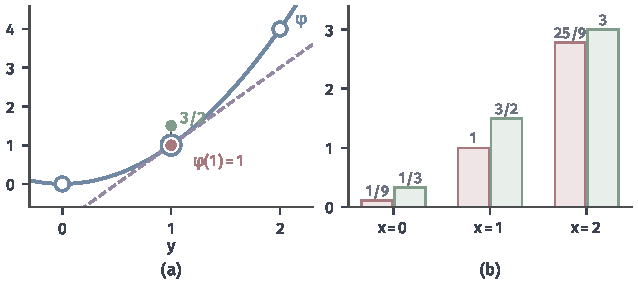
\includegraphics[width=108mm]{figures/07-probability/02-measure-theoretic-probability/matplotlib/cexp-jensen/figure.pdf}
  \caption{条件Jensen不等式，$\varphi(y)=y^{2}$，传感器表。(a)第二行$X=1$：空心圆是$(y,y^{2})$，大小与条件概率$\tfrac14,\tfrac12,\tfrac14$成正比；红点是$\varphi(\mathbb{E}[Y\mid X=1])=1$，绿点是$\mathbb{E}[Y^{2}\mid X=1]=3/2$，紫色虚线是$y=1$处的支撑线。(b)三行的$(\mathbb{E}[Y\mid X=x])^{2}$（红）与$\mathbb{E}[Y^{2}\mid X=x]$（绿）。}
  \label{fig:cexp-jensen}
\end{BookInlineFigure}

若$\varphi$是凹函数，对$-\varphi$用定理，不等号反向。例如对凹函数$-y^{2}$，得到的不等式两边乘以$-1$后就是上面的平方不等式。既不凸也不凹的函数没有确定的方向。取$\varphi(y)=y^{3}$，它在$[0,\infty)$上凸，在$(-\infty,0]$上凹。传感器表第一行中$Y$以$\tfrac23,\tfrac13$取$0,1$，两个值落在凸段上，
\[
 \bigl(\mathbb{E}[Y\mid X=0]\bigr)^{3}=\tfrac{1}{27}<\tfrac13=\mathbb{E}[Y^{3}\mid X=0].
\]
把变量平移成$Y-2$，第一行的两个值$-2,-1$落在凹段上，方向随之反转：
\[
 \bigl(\mathbb{E}[Y-2\mid X=0]\bigr)^{3}=-\tfrac{125}{27}\approx-4.63>-\tfrac{17}{3}\approx-5.67=\mathbb{E}\bigl[(Y-2)^{3}\bigm|X=0\bigr].
\]
同一个函数，作用在落于不同区段的取值上，可以给出相反的方向；只有在整个$\mathbb{R}$上凸，才能对一切变量和一切信息保证式~\eqref{eq:cexp-jensen}。

\subsection{\texorpdfstring{$L^p$}{Lp}收缩}
\label{sec:cexp-lp}

\paragraph{条件平均不放大\texorpdfstring{$L^{p}$}{Lp}范数}
对$1\leq p<\infty$，记
\[
 \lVert X\rVert_p=\bigl(\mathbb{E}\lvert X\rvert^{p}\bigr)^{1/p},
\]
$L^{p}$是满足$\lVert X\rVert_p<\infty$的随机变量组成的空间，两个几乎必然相等的随机变量视为同一个元素，见\BookChapterRef{chap:function-normed-spaces}{卷四第11章“赋范空间”}。在概率空间上，$L^{p}\subseteq L^{1}$：由逐点的不等式$\lvert x\rvert\leq1+\lvert x\rvert^{p}$取期望，得到$X$可积。再对凸函数$y\mapsto\lvert y\rvert^{p}$和可积的$\lvert X\rvert$用第~\ref{chap:random-variable-moments}章的Jensen不等式，
\[
 \bigl(\mathbb{E}\lvert X\rvert\bigr)^{p}\leq\mathbb{E}\lvert X\rvert^{p},
\]
即$\lVert X\rVert_1\leq\lVert X\rVert_p$。所以$L^{p}$中的随机变量都有条件期望。把条件Jensen不等式用于$\varphi(y)=\lvert y\rvert^{p}$，就得到条件期望对$L^{p}$范数的控制。

\begin{theorem}[\texorpdfstring{$L^{p}$}{Lp}收缩]
\label{thm:cexp-lp}
设$1\leq p<\infty$，$X\in L^{p}$。则$\mathbb{E}[X\mid\mathcal{G}]\in L^{p}$，并且
\begin{equation}
 \bigl\lVert\mathbb{E}[X\mid\mathcal{G}]\bigr\rVert_p\leq\lVert X\rVert_p .
 \label{eq:cexp-lp}
\end{equation}
\end{theorem}

\begin{proof}
$\varphi(y)=\lvert y\rvert^{p}$是$\mathbb{R}$上的凸函数，$X$与$\lvert X\rvert^{p}$都可积。由条件Jensen不等式，
\[
 \bigl\lvert\mathbb{E}[X\mid\mathcal{G}]\bigr\rvert^{p}\leq\mathbb{E}\bigl[\lvert X\rvert^{p}\bigm|\mathcal{G}\bigr].
\]
两边非负，取期望，右边由全期望公式等于$\mathbb{E}\lvert X\rvert^{p}$，于是
\[
 \mathbb{E}\bigl\lvert\mathbb{E}[X\mid\mathcal{G}]\bigr\rvert^{p}\leq\mathbb{E}\lvert X\rvert^{p}<\infty .
\]
两边开$p$次方即得。
\end{proof}

$p=\infty$的情形更直接：若$\lvert X\rvert\leq c$几乎必然成立，由保序，$\lvert\mathbb{E}[X\mid\mathcal{G}]\rvert\leq c$几乎必然成立。

\paragraph{对扰动的稳定性}
把定理用于两个输入之差。设$X_1,X_2\in L^{p}$，由线性，
\begin{equation}
 \bigl\lVert\mathbb{E}[X_1\mid\mathcal{G}]-\mathbb{E}[X_2\mid\mathcal{G}]\bigr\rVert_p\leq\lVert X_1-X_2\rVert_p .
 \label{eq:cexp-lp-stability}
\end{equation}
条件期望是$L^{p}$上的线性映射，范数不超过$1$：输入有一点扰动，输出的扰动不会更大。由此，若$X_n\to X$在$L^{p}$中成立，则$X_n$的条件期望也在$L^{p}$中收敛到$\mathbb{E}[X\mid\mathcal{G}]$，条件期望与$L^{p}$极限可以交换次序。

\paragraph{逐次等分的数值}
用逐次等分的例子观察这个不等式，把$X$中心化，取$X(\omega)=\omega^{2}-\tfrac13$。$n=1$时，两段上的平均是$\tfrac1{12}-\tfrac13$与$\tfrac{7}{12}-\tfrac13$，即
\[
 \mathbb{E}[X\mid\mathcal{G}_1]=-\tfrac14\ \text{在}\ [0,\tfrac12)\ \text{上},\qquad
 \mathbb{E}[X\mid\mathcal{G}_1]=\tfrac14\ \text{在}\ [\tfrac12,1)\ \text{上}.
\]
$\lvert\mathbb{E}[X\mid\mathcal{G}_1]\rvert$恒为$1/4$，所以它的各阶范数都是$1/4$。另一方面，$X$在$\omega_0=1/\sqrt3$处变号，分两段积分，
\[
 \lVert X\rVert_1=\int_0^{\omega_0}\Bigl(\frac13-\omega^{2}\Bigr)\mathrm{d}\omega+\int_{\omega_0}^{1}\Bigl(\omega^{2}-\frac13\Bigr)\mathrm{d}\omega=\frac{4}{9\sqrt3}\approx0.2566 .
\]
$\lVert X\rVert_2^{2}$是$\omega^{2}$的方差$\tfrac15-\tfrac19=\tfrac4{45}$，所以$\lVert X\rVert_2\approx0.2981$。两者都大于$1/4$，与式~\eqref{eq:cexp-lp}一致。

图~\ref{fig:cexp-lp-contraction}(a)画出$n=0,1,\dots,7$时$\lVert\mathbb{E}[X\mid\mathcal{G}_n]\rVert_p$，三条绿色折线分别对应$p=1,2,4$，都停在紫色虚线$\lVert X\rVert_p$之下。折线随$n$不减，这可以由塔式法则解释：$\mathcal{G}_n\subseteq\mathcal{G}_{n+1}$，由式~\eqref{eq:cexp-tower}，
\[
 \mathbb{E}[X\mid\mathcal{G}_n]=\mathbb{E}\bigl[\mathbb{E}[X\mid\mathcal{G}_{n+1}]\bigm|\mathcal{G}_n\bigr],
\]
把$\mathbb{E}[X\mid\mathcal{G}_{n+1}]$当作输入，对右边用式~\eqref{eq:cexp-lp}，得到
\[
 \bigl\lVert\mathbb{E}[X\mid\mathcal{G}_n]\bigr\rVert_p\leq\bigl\lVert\mathbb{E}[X\mid\mathcal{G}_{n+1}]\bigr\rVert_p .
\]
图中各折线还逐渐贴近上界。信息逐步增加时条件期望的收敛属于鞅的理论，可参考\BookChapterRef{chap:discrete-time-stochastic-processes}{卷九第3章“离散时间随机过程”}；这里只把它作为数值观察。

\begin{BookInlineFigure}
  \centering
  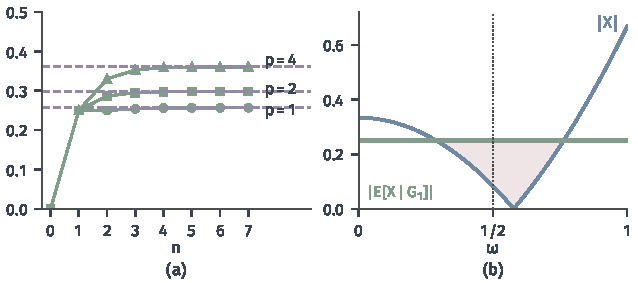
\includegraphics[width=108mm]{figures/07-probability/02-measure-theoretic-probability/matplotlib/cexp-lp-contraction/figure.pdf}
  \caption{$L^{p}$收缩，$\Omega=[0,1)$，$X(\omega)=\omega^{2}-\tfrac13$，$\mathcal{G}_n$由$2^{n}$个等长区间生成，范数用$2^{16}$个小区间上的中点公式计算。(a)$\lVert\mathbb{E}[X\mid\mathcal{G}_n]\rVert_p$（绿；圆、方、三角分别对应$p=1,2,4$）与$\lVert X\rVert_p$（紫色虚线）。(b)$n=1$时的$\lvert X\rvert$（蓝）与$\lvert\mathbb{E}[X\mid\mathcal{G}_1]\rvert$（绿），浅红区域上后者更大。}
  \label{fig:cexp-lp-contraction}
\end{BookInlineFigure}

\paragraph{控制的是总体大小}
式~\eqref{eq:cexp-lp}控制的是范数，即对整个$\Omega$平均后的大小，不是逐点的大小。图~\ref{fig:cexp-lp-contraction}(b)中，$\omega$在$\omega_0\approx0.577$附近时$\lvert X\rvert$接近$0$，而$\lvert\mathbb{E}[X\mid\mathcal{G}_1]\rvert=1/4$，浅红区域上条件平均的绝对值比原变量大。组内平均把组内的值拉向同一个数，原来接近零的样本点被拉离零，原来远离零的被拉近；拉近的部分在范数中占上风。传感器表中同样如此：格子$(0,0)$上$Y=0$，$\mathbb{E}[Y\mid X]=1/3$。


\section{最小均方预测}
\label{sec:cexp-prediction}

到目前为止，条件期望只被描述为“保留累计期望的组内平均”。它还有一个优化的含义：如果只能根据已知信息去猜$X$，并以平方误差的平均衡量猜得好坏，最好的猜法就是条件期望。第~\ref{chap:random-vectors}章在形如$a+bx$的直线中找过最好的预测，这里不限定形式，允许使用已知信息的任意函数，只要求预测量平方可积。

设$X$平方可积。一个只用$\mathcal{G}$中信息的预测量是一个$\mathcal{G}$可测的随机变量$W$，要求$\mathbb{E}[W^{2}]<\infty$；它的\term{均方误差}（mean squared error）是$\mathbb{E}[(X-W)^{2}]$。问题是：在所有这样的$W$中，哪一个使均方误差最小？卷四的Hilbert空间投影给出了现成的框架。

\subsection{正交投影}
\label{sec:cexp-projection}

\paragraph{预测量组成的子空间}
平方可积随机变量组成$L^{2}=L^{2}(\Omega,\mathcal{F},\mathbb{P})$，内积为$\langle U,V\rangle=\mathbb{E}[UV]$，范数为$\lVert U\rVert_2=(\mathbb{E}[U^{2}])^{1/2}$。卷四证明了$L^{2}$是Hilbert空间，并且对Hilbert空间的闭线性子空间$M$与任一元素$f$，$M$中离$f$最近的元素存在且唯一，它由“$f$减去它与$M$正交”刻画，可参考\BookChapterRef{chap:function-inner-product-spaces}{卷四第12章“内积空间”}。

记
\[
 L^{2}(\mathcal{G})=\bigl\{W\in L^{2}:\ W\ \text{几乎必然等于某个}\ \mathcal{G}\ \text{可测的随机变量}\bigr\}.
\]
它是全体候选预测量。均方误差$\mathbb{E}[(X-W)^{2}]$就是$\lVert X-W\rVert_2^{2}$，所以最小均方预测是在$L^{2}(\mathcal{G})$中找离$X$最近的点。要用投影定理，先确认这个集合是闭线性子空间。

\begin{lemma}[已知信息上的平方可积变量]
\label{lem:cexp-closed-subspace}
$L^{2}(\mathcal{G})$是$L^{2}$的闭线性子空间。
\end{lemma}

\begin{proof}
$\mathcal{G}$可测的函数的线性组合仍$\mathcal{G}$可测，所以$L^{2}(\mathcal{G})$是线性子空间。

闭性借助完备性。$L^{2}(\mathcal{G})$中的元素与概率空间$(\Omega,\mathcal{G},\mathbb{P}_{\mathcal{G}})$上的平方可积函数一一对应，并且对$\mathcal{G}$可测的函数，对$\mathbb{P}_{\mathcal{G}}$与对$\mathbb{P}$的积分相同（见定理~\ref{thm:cexp-existence}的证明），所以这一对应保持范数。$L^{2}(\Omega,\mathcal{G},\mathbb{P}_{\mathcal{G}})$本身是Hilbert空间，因而完备。设$W_n\in L^{2}(\mathcal{G})$在$L^{2}$中收敛到$W$，则$(W_n)$是Cauchy列，在$L^{2}(\Omega,\mathcal{G},\mathbb{P}_{\mathcal{G}})$中收敛到某个$\mathcal{G}$可测的$W'$，也就在$L^{2}$中收敛到$W'$。极限唯一，$W=W'$几乎必然成立，所以$W\in L^{2}(\mathcal{G})$。
\end{proof}

这里不能简单地说“$\mathcal{G}$可测函数的极限仍$\mathcal{G}$可测”：$L^{2}$收敛只给出一个子列几乎必然收敛，而例外的零概率集未必属于$\mathcal{G}$。借助完备性绕开了这个问题。

\paragraph{残差与已知信息正交}
现在说明条件期望正是投影。思路是：把式~\eqref{eq:cexp-defining}中的示性函数$\mathbf{1}_{A}$换成一般的$W\in L^{2}(\mathcal{G})$。

\begin{theorem}[条件期望是正交投影]
\label{thm:cexp-projection}
设$X\in L^{2}$。则$\mathbb{E}[X\mid\mathcal{G}]\in L^{2}(\mathcal{G})$，并且对每个$W\in L^{2}(\mathcal{G})$，
\begin{equation}
 \mathbb{E}\bigl[(X-\mathbb{E}[X\mid\mathcal{G}])\,W\bigr]=0 .
 \label{eq:cexp-orthogonality}
\end{equation}
因此$\mathbb{E}[X\mid\mathcal{G}]$是$X$在$L^{2}(\mathcal{G})$上的正交投影。
\end{theorem}

\begin{proof}
记$Z=\mathbb{E}[X\mid\mathcal{G}]$。由定理~\ref{thm:cexp-lp}取$p=2$，$Z\in L^{2}$，它又是$\mathcal{G}$可测的，所以$Z\in L^{2}(\mathcal{G})$。

取$W\in L^{2}(\mathcal{G})$，不妨设$W$本身$\mathcal{G}$可测。由Cauchy--Schwarz不等式，
\[
 \mathbb{E}\lvert WX\rvert\leq\lVert W\rVert_2\lVert X\rVert_2<\infty ,
\]
所以$WX$可积。由提取已知量，$\mathbb{E}[WX\mid\mathcal{G}]=WZ$；两边取期望，由全期望公式，
\[
 \mathbb{E}[WX]=\mathbb{E}\bigl[\mathbb{E}[WX\mid\mathcal{G}]\bigr]=\mathbb{E}[WZ] .
\]
移项即得式~\eqref{eq:cexp-orthogonality}。$X-Z$与闭子空间$L^{2}(\mathcal{G})$正交，而$Z$在这个子空间中，由卷四的正交刻画，$Z$是$X$在其上的正交投影。
\end{proof}

正交条件~\eqref{eq:cexp-orthogonality}是积分刻画的推广。取$W=\mathbf{1}_{A}$，$A\in\mathcal{G}$，它就是式~\eqref{eq:cexp-defining}：残差$X-Z$在每个已知事件上的累计为零。反过来，若某个$Z\in L^{2}(\mathcal{G})$满足正交条件，取$W=\mathbf{1}_{A}$就知道它满足条件期望的定义。所以对平方可积的$X$，投影定理本身就给出了条件期望的存在性，不必经过Radon--Nikodym定理。这条路线只覆盖平方可积的情形；对只可积的$X$，存在性仍由定理~\ref{thm:cexp-existence}保证。

\paragraph{传感器表中的投影}
传感器表把这幅几何图景变成了有限维的计算。七个正概率格子上的函数组成一个七维空间，内积是按格子概率加权的乘积和。$\sigma(X)$可测的函数是在每行取常数的函数，组成一个三维子空间。$Y$在它上面的投影就是按行平均，残差$Y-\mathbb{E}[Y\mid X]$在每行内的加权和为零，因而与每一个行常数函数正交。

勾股定理给出平方长度的拆分。记$m(X)=\mathbb{E}[Y\mid X]$，第~\ref{chap:random-vectors}章已算得$\operatorname{Var}(Y)=0.6$、$\operatorname{Var}(m(X))=4/15$、平均条件方差为$1/3$，于是
\[
 \mathbb{E}[Y^{2}]=1.6,\qquad \mathbb{E}\bigl[m(X)^{2}\bigr]=\tfrac{4}{15}+1=\tfrac{19}{15},\qquad \mathbb{E}\bigl[(Y-m(X))^{2}\bigr]=\tfrac13 ,
\]
并且$\tfrac{19}{15}+\tfrac{5}{15}=\tfrac{24}{15}=1.6$。图~\ref{fig:cexp-projection}是这一关系的示意：$X$到平面$L^{2}(\mathcal{G})$的垂线足是$\mathbb{E}[X\mid\mathcal{G}]$。

\begin{BookInlineFigure}
  \centering
  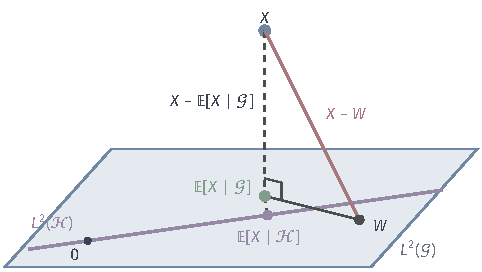
\includegraphics[width=82mm]{figures/07-probability/02-measure-theoretic-probability/tikz/cexp-projection/figure.pdf}
  \caption{条件期望是正交投影（示意）。浅蓝平面是$L^{2}(\mathcal{G})$，平面内的紫线是较小信息$\mathcal{H}\subseteq\mathcal{G}$对应的$L^{2}(\mathcal{H})$，常数（含$0$）都在其中。$X$的垂线足是$\mathbb{E}[X\mid\mathcal{G}]$（绿），残差（虚线）与平面垂直；平面中另一点$W$与$X$的距离（红）更长。再把$\mathbb{E}[X\mid\mathcal{G}]$投影到紫线上，得到$\mathbb{E}[X\mid\mathcal{H}]$。}
  \label{fig:cexp-projection}
\end{BookInlineFigure}

投影的观点也解释了塔式法则。$\mathcal{H}\subseteq\mathcal{G}$时$L^{2}(\mathcal{H})\subseteq L^{2}(\mathcal{G})$，先投影到大的子空间再投影到小的子空间，等于直接投影到小的子空间；先投影到小的子空间，结果已在大的子空间中，再投影到大的子空间不改变它。这正是式~\eqref{eq:cexp-tower}的两个等号在平方可积情形的几何含义。

\subsection{平方误差分解}
\label{sec:cexp-mse}

\paragraph{误差的勾股定理}
正交性直接给出任一预测量的误差构成。

\begin{theorem}[平方误差分解]
\label{thm:cexp-mse}
设$X\in L^{2}$，$Z=\mathbb{E}[X\mid\mathcal{G}]$。对每个$W\in L^{2}(\mathcal{G})$，
\begin{equation}
 \mathbb{E}\bigl[(X-W)^{2}\bigr]=\mathbb{E}\bigl[(X-Z)^{2}\bigr]+\mathbb{E}\bigl[(Z-W)^{2}\bigr].
 \label{eq:cexp-mse}
\end{equation}
因此$Z$在$L^{2}(\mathcal{G})$中使均方误差最小，并且使均方误差最小的$W$几乎必然等于$Z$。
\end{theorem}

\begin{proof}
把预测误差拆成两段：
\[
 X-W=(X-Z)+(Z-W).
\]
平方后取期望，交叉项是$2\,\mathbb{E}[(X-Z)(Z-W)]$。$Z-W\in L^{2}(\mathcal{G})$，由式~\eqref{eq:cexp-orthogonality}，交叉项为零，得到式~\eqref{eq:cexp-mse}。右边第二项非负，所以$\mathbb{E}[(X-W)^{2}]\geq\mathbb{E}[(X-Z)^{2}]$；等号成立当且仅当$\mathbb{E}[(Z-W)^{2}]=0$，即$W=Z$几乎必然成立。
\end{proof}

式~\eqref{eq:cexp-mse}把误差分成两部分：$\mathbb{E}[(X-Z)^{2}]$是已知信息无论如何也消除不了的部分，与$W$无关；$\mathbb{E}[(Z-W)^{2}]$是$W$偏离最佳预测而多付的代价。

用传感器表演示。取$\mathcal{G}=\sigma(X)$，再取一个较差的预测$W=\mathbb{E}[Y\mid\mathcal{H}]$，$\mathcal{H}=\sigma(\mathbf{1}_{\{X=2\}})$。它在前两行取$5/7$、第三行取$5/3$，是行常数函数，属于$L^{2}(\sigma(X))$。按行计算多付的代价：
\[
 \mathbb{E}\bigl[(Z-W)^{2}\bigr]=0.3\Bigl(\frac13-\frac57\Bigr)^{2}+0.4\Bigl(1-\frac57\Bigr)^{2}+0.3\cdot0=\frac{64}{1470}+\frac{16}{490}=\frac{8}{105}.
\]
再加上不可消除的部分$1/3$，
\[
 \mathbb{E}\bigl[(Y-W)^{2}\bigr]=\frac13+\frac{8}{105}=\frac{43}{105}\approx0.410 .
\]
直接按格子计算$(Y-W)^{2}$的加权和，也得到$43/105$。

\paragraph{信息多了，误差平均不增}
若$\mathcal{H}\subseteq\mathcal{G}$，则$\mathbb{E}[X\mid\mathcal{H}]\in L^{2}(\mathcal{H})\subseteq L^{2}(\mathcal{G})$，可以取它作为式~\eqref{eq:cexp-mse}中的$W$，得到
\begin{equation}
 \mathbb{E}\bigl[(X-\mathbb{E}[X\mid\mathcal{H}])^{2}\bigr]=\mathbb{E}\bigl[(X-\mathbb{E}[X\mid\mathcal{G}])^{2}\bigr]+\mathbb{E}\bigl[(\mathbb{E}[X\mid\mathcal{G}]-\mathbb{E}[X\mid\mathcal{H}])^{2}\bigr].
 \label{eq:cexp-information-monotone}
\end{equation}
更多的信息使最小均方误差不增，减少的量恰好是两个最佳预测之差的平方平均。上面的数值正是这一式的例子：只知道“是否偏高”时最小误差是$43/105$，知道完整的第一台读数后降到$1/3$。

这只是平均意义下的结论，不是逐个样本点的结论。图~\ref{fig:cexp-pointwise-error}比较七个正概率格子上的平方误差。格子$(0,1)$上$Y=1$，较粗的预测$5/7$误差为$4/49\approx0.08$，较细的预测$1/3$误差为$4/9\approx0.44$；格子$(1,0)$上误差也从约$0.51$增到$1$。信息变多后，这两个格子的预测变差了；但其他格子的改善更多，按概率加权后总体误差从$0.410$降到$0.333$。

\begin{BookInlineFigure}
  \centering
  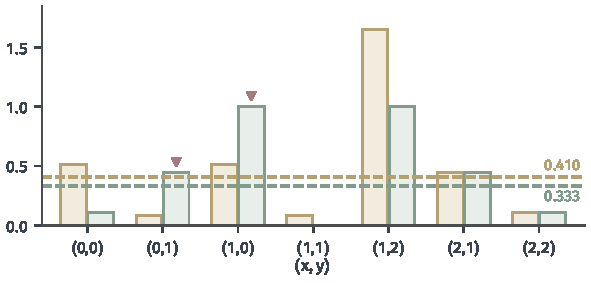
\includegraphics[width=100mm]{figures/07-probability/02-measure-theoretic-probability/matplotlib/cexp-pointwise-error/figure.pdf}
  \caption{逐格的平方误差，传感器表的七个正概率格子。黄柱：用$\mathbb{E}[Y\mid\mathcal{H}]$预测，$\mathcal{H}=\sigma(\mathbf{1}_{\{X=2\}})$；绿柱：用$\mathbb{E}[Y\mid X]$预测。红色三角标出信息增加后误差变大的格子$(0,1)$与$(1,0)$；两条虚线是按概率加权的平均误差$43/105\approx0.410$与$1/3$。}
  \label{fig:cexp-pointwise-error}
\end{BookInlineFigure}

最小化是在所有$\mathcal{G}$可测的平方可积预测量中进行的，不限于线性函数。传感器表与三角形模型中，$\mathbb{E}[Y\mid X]$恰好是$X$的线性函数，所以第~\ref{chap:random-vectors}章的最佳直线与这里的最佳预测重合。“只知绝对值”的例子中，$\mathrm{e}^{X}$的最佳预测$\cosh\lvert X\rvert$不是$\lvert X\rvert$的线性函数，最佳直线的均方误差就严格大于最佳预测的均方误差。从样本中估计这样的预测函数是统计推断的问题，可参考\BookChapterRef{chap:nonparametric-inference}{卷八第2章“非参数分布与函数推断”}。

\subsection{条件方差与全方差公式}
\label{sec:cexp-conditional-variance}

\paragraph{条件方差}
最小误差$\mathbb{E}[(X-Z)^{2}]$是一个数，它是对整个$\Omega$平均的结果。在每个已知群体内，残差平方的平均可以不同：传感器表中，第一行与第三行的条件方差是$2/9$，第二行是$1/2$。把残差平方再给定$\mathcal{G}$求条件期望，就得到随已知信息变化的波动大小。

\begin{definition}[条件方差]
\label{def:cexp-conditional-variance}
设$X\in L^{2}$，$Z=\mathbb{E}[X\mid\mathcal{G}]$。称
\begin{equation}
 \operatorname{Var}(X\mid\mathcal{G})=\mathbb{E}\bigl[(X-Z)^{2}\bigm|\mathcal{G}\bigr]
 \label{eq:cexp-conditional-variance}
\end{equation}
为$X$给定$\mathcal{G}$的条件方差。给定随机对象$Y$时取$\mathcal{G}=\sigma(Y)$，记作$\operatorname{Var}(X\mid Y)$。
\end{definition}

$(X-Z)^{2}$可积，因为$X,Z\in L^{2}$，所以定义有意义。它是$\mathcal{G}$可测的非负随机变量，只确定到零概率集。给定离散或有密度的$Y$时，第~\ref{chap:random-vectors}章的$v(y)=\operatorname{Var}(X\mid Y=y)$经过复合得到它的一个版本，理由与第~\ref{sec:cexp-given-variable}节的条件均值相同。

与不带条件的方差一样，条件方差有二阶矩的写法：
\begin{equation}
 \operatorname{Var}(X\mid\mathcal{G})=\mathbb{E}[X^{2}\mid\mathcal{G}]-\bigl(\mathbb{E}[X\mid\mathcal{G}]\bigr)^{2}.
 \label{eq:cexp-conditional-variance-moment}
\end{equation}
推导时把平方展开，$(X-Z)^{2}=X^{2}-2XZ+Z^{2}$，三项都可积，其中$XZ$的可积性由Cauchy--Schwarz不等式保证。对三项分别求条件期望，$Z$是已知量，由提取已知量，
\[
 \mathbb{E}[XZ\mid\mathcal{G}]=Z\,\mathbb{E}[X\mid\mathcal{G}]=Z^{2},\qquad \mathbb{E}[Z^{2}\mid\mathcal{G}]=Z^{2}.
\]
再由线性，
\[
 \operatorname{Var}(X\mid\mathcal{G})=\mathbb{E}[X^{2}\mid\mathcal{G}]-2Z^{2}+Z^{2}=\mathbb{E}[X^{2}\mid\mathcal{G}]-Z^{2}.
\]
由条件Jensen不等式，右边几乎必然非负，与定义一致。传感器表中，由第~\ref{sec:cexp-known}节的$\mathbb{E}[Y^{2}\mid X]$，第二行为$\tfrac32-1^{2}=\tfrac12$。

\needspace{8\baselineskip}
\paragraph{全方差公式}
有了条件方差，总方差可以拆成两部分。

\begin{theorem}[全方差公式]
\label{thm:cexp-total-variance}
设$X\in L^{2}$。则
\begin{equation}
 \operatorname{Var}(X)=\mathbb{E}\bigl[\operatorname{Var}(X\mid\mathcal{G})\bigr]+\operatorname{Var}\bigl(\mathbb{E}[X\mid\mathcal{G}]\bigr).
 \label{eq:cexp-total-variance}
\end{equation}
\end{theorem}

\begin{proof}
记$Z=\mathbb{E}[X\mid\mathcal{G}]$。常数$\mathbb{E}[X]$属于$L^{2}(\mathcal{G})$，在式~\eqref{eq:cexp-mse}中取$W=\mathbb{E}[X]$，
\[
 \mathbb{E}\bigl[(X-\mathbb{E}[X])^{2}\bigr]=\mathbb{E}\bigl[(X-Z)^{2}\bigr]+\mathbb{E}\bigl[(Z-\mathbb{E}[X])^{2}\bigr].
\]
左边是$\operatorname{Var}(X)$。右边第一项由全期望公式与式~\eqref{eq:cexp-conditional-variance}，
\[
 \mathbb{E}\bigl[(X-Z)^{2}\bigr]=\mathbb{E}\Bigl[\mathbb{E}\bigl[(X-Z)^{2}\bigm|\mathcal{G}\bigr]\Bigr]=\mathbb{E}\bigl[\operatorname{Var}(X\mid\mathcal{G})\bigr].
\]
由全期望公式$\mathbb{E}[Z]=\mathbb{E}[X]$，所以第二项是$\operatorname{Var}(Z)$。
\end{proof}

第一项是组内波动的平均，第二项是各组平均之间的波动。第~\ref{chap:random-vectors}章对概率表和联合密度分别证明过这个公式，现在它对任何信息都成立，证明只用到正交分解。

\paragraph{信息怎样重新分配方差}
总方差是固定的，信息只是在两项之间重新分配。图~\ref{fig:cexp-information-variance}(a)对传感器表的四层信息
\[
 \{\emptyset,\Omega\}\subseteq\mathcal{H}\subseteq\sigma(X)\subseteq\sigma(X,Y)
\]
画出这一分配。什么也不知道时，全部$0.6$都是组内波动；知道“是否偏高”时拆成$\tfrac{43}{105}+\tfrac{4}{21}$；知道第一台读数时拆成$\tfrac13+\tfrac{4}{15}$；知道两台读数时$Y$已知，全部是组间波动。由式~\eqref{eq:cexp-information-monotone}，组内波动的平均随信息增加而不增。$\mathcal{H}$这一层的组间部分可以直接算：$\mathbb{E}[Y\mid\mathcal{H}]$以概率$0.7,0.3$取$5/7,5/3$，均值为$1$，
\[
 \operatorname{Var}\bigl(\mathbb{E}[Y\mid\mathcal{H}]\bigr)=0.7\Bigl(\frac57-1\Bigr)^{2}+0.3\Bigl(\frac53-1\Bigr)^{2}=\frac{2}{35}+\frac{2}{15}=\frac{4}{21}.
\]

\begin{BookInlineFigure}
  \centering
  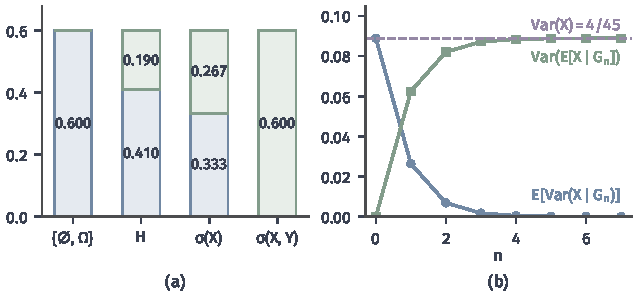
\includegraphics[width=108mm]{figures/07-probability/02-measure-theoretic-probability/matplotlib/cexp-information-variance/figure.pdf}
  \caption{全方差公式在信息增加时的分配。浅蓝或蓝色表示$\mathbb{E}[\operatorname{Var}(\cdot\mid\mathcal{G})]$，浅绿或绿色表示$\operatorname{Var}(\mathbb{E}[\cdot\mid\mathcal{G}])$。(a)传感器表中$Y$的方差$0.6$在四层信息下的拆分，$\mathcal{H}=\sigma(\mathbf{1}_{\{X=2\}})$。(b)$\Omega=[0,1)$，$X(\omega)=\omega^{2}$，$\mathcal{G}_n$为$2^{n}$等分，两部分之和恒为$\operatorname{Var}(X)=4/45$（紫色虚线）。}
  \label{fig:cexp-information-variance}
\end{BookInlineFigure}

逐次等分的例子给出一个连续的版本，见图~\ref{fig:cexp-information-variance}(b)。这里$X$的二阶矩是$\int_0^1\omega^{4}\,\mathrm{d}\omega=\tfrac15$，均值是$\tfrac13$，方差为$\tfrac15-\tfrac19=\tfrac4{45}$。$n=1$时，$\mathbb{E}[X\mid\mathcal{G}_1]$以各$\tfrac12$的概率取$\tfrac1{12}$与$\tfrac7{12}$，与均值$\tfrac13$各差$\tfrac14$，所以
\[
 \operatorname{Var}\bigl(\mathbb{E}[X\mid\mathcal{G}_1]\bigr)=\frac1{16},\qquad
 \mathbb{E}\bigl[\operatorname{Var}(X\mid\mathcal{G}_1)\bigr]=\frac4{45}-\frac1{16}=\frac{19}{720}\approx0.0264 .
\]
随着$n$增大，组间部分逐渐占据几乎全部方差，组内部分趋于零：分得越细，每段内$\omega^{2}$的变化越小。

\paragraph{平均下降，个别组可以上升}
与误差一样，“组内波动不增”只对平均成立。按读数之差$D$分组时，$\{D=0\}$组内$Y$等可能取$0,1,2$，
\[
 \operatorname{Var}(Y\mid D=0)=\frac{0+1+4}{3}-1^{2}=\frac23>0.6=\operatorname{Var}(Y).
\]
知道两台读数一致以后，第二台读数的波动反而比不加条件时更大；这一组的波动由另外两组较小的波动平衡，平均条件方差仍不超过$0.6$。


\section{本章小结}
\label{sec:cexp-summary}

本章从一个现有公式算不出的问题出发：只知道$\lvert X\rvert$时，$X^{+}$的平均是多少。每个条件事件的概率都是零，没有概率表也没有联合密度，组内平均无从相除。解决的办法是换一种描述：不再除以组的概率，而是要求条件平均只用已知信息，并在每个已知事件上保留原变量的累计期望。有限分组时，这两条要求恰好刻画了组内平均；一般信息下，它们就是条件期望的定义，“只知绝对值”的答案$\lvert X\rvert/2$由它直接验证。

这个定义总有解，而且解只确定到零概率集。存在性来自Radon--Nikodym定理：把$A\mapsto\mathbb{E}[X\mathbf{1}_{A}]$看作已知事件上的测度，条件期望就是它相对于$\mathbb{P}$、并且只用已知信息的密度。唯一性只用到积分定义在足够多的事件上成立。给定观测$Y$时，条件期望可以写成$m(Y)$，但函数$m$只在$Y$的分布下几乎处处确定；单个零概率观测值上的条件平均不由定义决定，要在第~\ref{chap:conditional-distributions}章借助额外的结构处理。

所有运算规则都从积分定义核验，并且都按几乎必然理解。表~\ref{tab:cexp-summary}按传感器表汇总了这些规则、它们需要的条件和例中的数值。

\begin{BookInlineTable}
  \centering
  \caption{条件期望的规则（传感器表，$m(X)=\mathbb{E}[Y\mid X]$）}
  \label{tab:cexp-summary}
  \begin{tabular}{lll}
    \toprule
    规则 & 条件 & 例中的数值 \\
    \midrule
    线性与保序 & 各变量可积 & $\mathbb{E}[2Y-1\mid X]=2m(X)-1$ \\
    提取已知量 & $H$已知，$X$与$HX$可积 & $\mathbb{E}[XY\mid X=2]=\tfrac{10}{3}$ \\
    独立的信息 & $X$与$\mathcal{G}$独立 & $\mathbb{E}[\operatorname{sgn}X\mid\lvert X\rvert]=0$ \\
    全期望公式 & $X$可积 & $0.3\cdot\tfrac13+0.4+0.3\cdot\tfrac53=1$ \\
    塔式法则 & $\mathcal{H}\subseteq\mathcal{G}$ & $\{X\leq1\}$上为$\tfrac57$ \\
    条件Jensen & $\varphi$凸，$X$与$\varphi(X)$可积 & $1\leq\mathbb{E}[Y^{2}\mid X=1]=\tfrac32$ \\
    $L^{p}$收缩 & $X\in L^{p}$，$1\leq p<\infty$ & 范数不增，逐点可增 \\
    最小均方预测 & $X\in L^{2}$ & 最小误差$\tfrac13<\tfrac{43}{105}$ \\
    全方差公式 & $X\in L^{2}$ & $0.6=\tfrac13+\tfrac{4}{15}$ \\
    \bottomrule
  \end{tabular}
\end{BookInlineTable}

规则的边界同样重要。只有已知的乘子能提到条件期望之外。条件平均为常数不能推出独立，它只约束一个平均值，不约束整个条件规律。迭代条件期望只有在两份信息有包含关系时才能化简，结果总是较粗的那一层；互不包含时两种顺序的结果不同，也不等于共同信息上的平均。凸性决定Jensen不等式的方向，证明中只能使用可数条支撑线，以便合并例外的零概率集。

条件期望的条件有两个层次。积分定义、存在唯一性、运算规则、迭代和Jensen不等式只要求可积；最小均方预测、正交投影、条件方差和全方差公式要求平方可积。在平方可积的情形，条件期望是$L^{2}$中到已知信息子空间的正交投影，塔式法则是逐次投影，全方差公式是勾股定理。信息越多，最小均方误差与平均条件方差越小，但这只是平均意义下的结论，个别样本点上的误差和个别组的条件方差都可能变大。

本章只为每个可积变量求条件平均。对每个事件$\{X\in B\}$的示性函数求条件期望，得到一族条件概率；把这一族组织成对每个观测值都是概率分布的对象，就是第~\ref{chap:conditional-distributions}章的条件分布，那里再说明条件期望怎样写成对条件分布的积分。信息随时间逐步增加、一列条件期望怎样演化，则属于随机过程的研究。

